% Options for packages loaded elsewhere
\PassOptionsToPackage{unicode}{hyperref}
\PassOptionsToPackage{hyphens}{url}
\PassOptionsToPackage{dvipsnames,svgnames,x11names}{xcolor}
\documentclass[
  10pt,
]{extarticle}
\usepackage{xcolor}
\usepackage[top=1.5in, bottom=1.5in, left=1.5in, right=1.5in]{geometry}
\usepackage{amsmath,amssymb}
\setcounter{secnumdepth}{5}
\usepackage{iftex}
\ifPDFTeX
  \usepackage[T1]{fontenc}
  \usepackage[utf8]{inputenc}
  \usepackage{textcomp} % provide euro and other symbols
\else % if luatex or xetex
  \usepackage{unicode-math} % this also loads fontspec
  \defaultfontfeatures{Scale=MatchLowercase}
  \defaultfontfeatures[\rmfamily]{Ligatures=TeX,Scale=1}
\fi
\usepackage{lmodern}
\ifPDFTeX\else
  % xetex/luatex font selection
\fi
% Use upquote if available, for straight quotes in verbatim environments
\IfFileExists{upquote.sty}{\usepackage{upquote}}{}
\IfFileExists{microtype.sty}{% use microtype if available
  \usepackage[]{microtype}
  \UseMicrotypeSet[protrusion]{basicmath} % disable protrusion for tt fonts
}{}
\makeatletter
\@ifundefined{KOMAClassName}{% if non-KOMA class
  \IfFileExists{parskip.sty}{%
    \usepackage{parskip}
  }{% else
    \setlength{\parindent}{0pt}
    \setlength{\parskip}{6pt plus 2pt minus 1pt}}
}{% if KOMA class
  \KOMAoptions{parskip=half}}
\makeatother
\usepackage{color}
\usepackage{fancyvrb}
\newcommand{\VerbBar}{|}
\newcommand{\VERB}{\Verb[commandchars=\\\{\}]}
\DefineVerbatimEnvironment{Highlighting}{Verbatim}{commandchars=\\\{\}}
% Add ',fontsize=\small' for more characters per line
\usepackage{framed}
\definecolor{shadecolor}{RGB}{248,248,248}
\newenvironment{Shaded}{\begin{snugshade}}{\end{snugshade}}
\newcommand{\AlertTok}[1]{\textcolor[rgb]{0.94,0.16,0.16}{#1}}
\newcommand{\AnnotationTok}[1]{\textcolor[rgb]{0.56,0.35,0.01}{\textbf{\textit{#1}}}}
\newcommand{\AttributeTok}[1]{\textcolor[rgb]{0.13,0.29,0.53}{#1}}
\newcommand{\BaseNTok}[1]{\textcolor[rgb]{0.00,0.00,0.81}{#1}}
\newcommand{\BuiltInTok}[1]{#1}
\newcommand{\CharTok}[1]{\textcolor[rgb]{0.31,0.60,0.02}{#1}}
\newcommand{\CommentTok}[1]{\textcolor[rgb]{0.56,0.35,0.01}{\textit{#1}}}
\newcommand{\CommentVarTok}[1]{\textcolor[rgb]{0.56,0.35,0.01}{\textbf{\textit{#1}}}}
\newcommand{\ConstantTok}[1]{\textcolor[rgb]{0.56,0.35,0.01}{#1}}
\newcommand{\ControlFlowTok}[1]{\textcolor[rgb]{0.13,0.29,0.53}{\textbf{#1}}}
\newcommand{\DataTypeTok}[1]{\textcolor[rgb]{0.13,0.29,0.53}{#1}}
\newcommand{\DecValTok}[1]{\textcolor[rgb]{0.00,0.00,0.81}{#1}}
\newcommand{\DocumentationTok}[1]{\textcolor[rgb]{0.56,0.35,0.01}{\textbf{\textit{#1}}}}
\newcommand{\ErrorTok}[1]{\textcolor[rgb]{0.64,0.00,0.00}{\textbf{#1}}}
\newcommand{\ExtensionTok}[1]{#1}
\newcommand{\FloatTok}[1]{\textcolor[rgb]{0.00,0.00,0.81}{#1}}
\newcommand{\FunctionTok}[1]{\textcolor[rgb]{0.13,0.29,0.53}{\textbf{#1}}}
\newcommand{\ImportTok}[1]{#1}
\newcommand{\InformationTok}[1]{\textcolor[rgb]{0.56,0.35,0.01}{\textbf{\textit{#1}}}}
\newcommand{\KeywordTok}[1]{\textcolor[rgb]{0.13,0.29,0.53}{\textbf{#1}}}
\newcommand{\NormalTok}[1]{#1}
\newcommand{\OperatorTok}[1]{\textcolor[rgb]{0.81,0.36,0.00}{\textbf{#1}}}
\newcommand{\OtherTok}[1]{\textcolor[rgb]{0.56,0.35,0.01}{#1}}
\newcommand{\PreprocessorTok}[1]{\textcolor[rgb]{0.56,0.35,0.01}{\textit{#1}}}
\newcommand{\RegionMarkerTok}[1]{#1}
\newcommand{\SpecialCharTok}[1]{\textcolor[rgb]{0.81,0.36,0.00}{\textbf{#1}}}
\newcommand{\SpecialStringTok}[1]{\textcolor[rgb]{0.31,0.60,0.02}{#1}}
\newcommand{\StringTok}[1]{\textcolor[rgb]{0.31,0.60,0.02}{#1}}
\newcommand{\VariableTok}[1]{\textcolor[rgb]{0.00,0.00,0.00}{#1}}
\newcommand{\VerbatimStringTok}[1]{\textcolor[rgb]{0.31,0.60,0.02}{#1}}
\newcommand{\WarningTok}[1]{\textcolor[rgb]{0.56,0.35,0.01}{\textbf{\textit{#1}}}}
\usepackage{longtable,booktabs,array}
\newcounter{none} % for unnumbered tables
\usepackage{calc} % for calculating minipage widths
% Correct order of tables after \paragraph or \subparagraph
\usepackage{etoolbox}
\makeatletter
\patchcmd\longtable{\par}{\if@noskipsec\mbox{}\fi\par}{}{}
\makeatother
% Allow footnotes in longtable head/foot
\IfFileExists{footnotehyper.sty}{\usepackage{footnotehyper}}{\usepackage{footnote}}
\makesavenoteenv{longtable}
\usepackage{graphicx}
\makeatletter
\newsavebox\pandoc@box
\newcommand*\pandocbounded[1]{% scales image to fit in text height/width
  \sbox\pandoc@box{#1}%
  \Gscale@div\@tempa{\textheight}{\dimexpr\ht\pandoc@box+\dp\pandoc@box\relax}%
  \Gscale@div\@tempb{\linewidth}{\wd\pandoc@box}%
  \ifdim\@tempb\p@<\@tempa\p@\let\@tempa\@tempb\fi% select the smaller of both
  \ifdim\@tempa\p@<\p@\scalebox{\@tempa}{\usebox\pandoc@box}%
  \else\usebox{\pandoc@box}%
  \fi%
}
% Set default figure placement to htbp
\def\fps@figure{htbp}
\makeatother
\setlength{\emergencystretch}{3em} % prevent overfull lines
\providecommand{\tightlist}{%
  \setlength{\itemsep}{0pt}\setlength{\parskip}{0pt}}
\usepackage{xcolor}
\usepackage{hyperref}
\hypersetup{colorlinks=true, linkcolor=blue, urlcolor=blue, citecolor=blue}
\usepackage{float}
\usepackage{fvextra}
\usepackage{fancyhdr}
\usepackage{lastpage}
\usepackage{soul}
\usepackage{etoolbox}
\usepackage{microtype}
\usepackage{tcolorbox}
\usepackage{enumitem}
\usepackage{fancyvrb}
\usepackage{xspace}
\allowdisplaybreaks
\setcounter{tocdepth}{2}
\setcounter{secnumdepth}{0}
\floatplacement{figure}{H}
\makeatletter
\newcommand{\@subtitle}{}
\newcommand{\subtitle}[1]{\gdef\@subtitle{#1}}
\newcommand{\DocSubtitle}{\@subtitle}
\renewcommand{\maketitle}{
  \thispagestyle{plain}
  \null
  \vfill
  \begin{center}
    {\Large \textsc{\@title} \par}\vskip 0.5em
    {\LARGE \bfseries \@subtitle \par}\vskip 0.75em
    {\large \@author \par}\vskip 0.5em
    {\normalsize \@date \par}
  \end{center}
  \vfill
  \tableofcontents
  \vspace{1em}
  \clearpage
}
\AfterEndEnvironment{Highlighting}{\setcounter{CodeLine}{\numexpr\value{CodeLine}+\FV@CodeLineNo\relax}}
\makeatother
\fancypagestyle{plain}{
  \fancyhf{}
  \renewcommand{\headrulewidth}{0pt}
  \renewcommand{\footrulewidth}{0pt}
}
\pagestyle{fancy}
\fancyhf{}
\fancyfoot[C]{\small\textsc{Page}~\thepage~\textsc{of}~\pageref{LastPage}}
\fancyhead[L]{\textsc{Rento Saijo}}
\fancyhead[R]{\textsc{\DocSubtitle}}
\fancyhead[C]{\textsc{\rightmark}}
\renewcommand{\headrulewidth}{0.5pt}
\renewcommand{\footrulewidth}{0.5pt}
\newcounter{CodeLine}
\newcounter{cell}
\AtBeginEnvironment{Highlighting}{\stepcounter{cell}}
\DefineVerbatimEnvironment{Highlighting}{Verbatim}{
  frame=single,
  rulecolor=\color{black},
  framesep=2mm,
  label=\footnotesize Cell \thecell,
  labelposition=topline,
  commandchars=\\\{\},
  breaklines=true,
  breakanywhere=false,
  breaksymbol={},
  numbers=left,
  numbersep=3pt,
  firstnumber=\numexpr\value{CodeLine}+1\relax,
  fontsize=\small
}
\DefineVerbatimEnvironment{verbatim}{Verbatim}{
  breaklines=true,
  breakanywhere=true,
  numbers=left,
  numbersep=3pt,
  firstnumber=1,
  fontsize=\footnotesize
}
\newtcolorbox{problem}[1][]{
  title={\textsc{#1}}
}
\renewcommand{\contentsname}{Table of Contents}
\newcommand{\E}{\mathrm{E}}
\newcommand{\Var}{\mathrm{Var}}
\newcommand{\Cov}{\mathrm{Cov}}
\newcommand{\R}{\textsf{R}\xspace}
\newcommand{\SD}{\mathrm{SD}}
\newcommand{\SE}{\mathrm{SE}}
\usepackage{bookmark}
\IfFileExists{xurl.sty}{\usepackage{xurl}}{} % add URL line breaks if available
\urlstyle{same}
\hypersetup{
  pdftitle={STA 209: Introduction to Time Series Analysis},
  colorlinks=true,
  linkcolor={blue},
  filecolor={Maroon},
  citecolor={blue},
  urlcolor={blue},
  pdfcreator={LaTeX via pandoc}}

\title{STA 209: Introduction to Time Series Analysis}
\usepackage{etoolbox}
\makeatletter
\providecommand{\subtitle}[1]{% add subtitle to \maketitle
  \apptocmd{\@title}{\par {\large #1 \par}}{}{}
}
\makeatother
\subtitle{Homework 6}
\author{Rento Saijo}
\date{April 21, 2026}

\begin{document}
\maketitle

\section{Disclosure}\label{disclosure}

GPT-5.4 (High) on Codex was used to create the \texttt{YAML} portion and some \texttt{LaTeX} code to format the text and equations. Page-formatting code was also provided by Derin Gezgin. In the setup, chunk options were set for the document, and helper functions were defined for repetitive plotting and table-formatting steps. See the original \texttt{RMD} file \href{https://github.com/RentoSaijo/STA209/blob/main/Homework6.Rmd}{here} for more details.

\newpage

\section{Problem 1}\label{problem-1}

\begin{problem}[Problem 1]
The glacial varve record (\texttt{varve} in \texttt{astsa}) exhibits some non-stationarity that can be improved by transforming to logarithms and some additional non-stationarity that can be corrected by differencing the logarithms.
\end{problem}

\newpage

\subsection{Problem 1 (a)}\label{problem-1-a}

\begin{problem}[Problem 1 (a)]
Argue that the glacial varves series, say \(X_t\), exhibits heteroscedasticity by computing the sample variance over the first half and the second half of the data. Argue that the transformation \(Y_t=\log X_t\) stabilizes the variance over the series. Plot the histograms of \(X_t\) and \(Y_t\) to see whether the approximation to normality is improved by transforming the data (use histogram and QQ plots).
\end{problem}

\begin{Shaded}
\begin{Highlighting}[]
\CommentTok{\# Compute the first{-}half and second{-}half sample variances.}
\NormalTok{n\_varve }\OtherTok{\textless{}{-}} \FunctionTok{length}\NormalTok{(varve\_x)}
\NormalTok{half\_varve }\OtherTok{\textless{}{-}} \FunctionTok{floor}\NormalTok{(n\_varve }\SpecialCharTok{/} \DecValTok{2}\NormalTok{)}
\FunctionTok{data.frame}\NormalTok{(}
  \AttributeTok{Series =} \FunctionTok{c}\NormalTok{(}\StringTok{\textquotesingle{}X\_t\textquotesingle{}}\NormalTok{, }\StringTok{\textquotesingle{}Y\_t = log(X\_t)\textquotesingle{}}\NormalTok{),}
  \AttributeTok{First\_Half =} \FunctionTok{c}\NormalTok{(}\FunctionTok{var}\NormalTok{(varve\_x[}\DecValTok{1}\SpecialCharTok{:}\NormalTok{half\_varve]), }\FunctionTok{var}\NormalTok{(varve\_y[}\DecValTok{1}\SpecialCharTok{:}\NormalTok{half\_varve])),}
  \AttributeTok{Second\_Half =} \FunctionTok{c}\NormalTok{(}\FunctionTok{var}\NormalTok{(varve\_x[(half\_varve }\SpecialCharTok{+} \DecValTok{1}\NormalTok{)}\SpecialCharTok{:}\NormalTok{n\_varve]), }\FunctionTok{var}\NormalTok{(varve\_y[(half\_varve }\SpecialCharTok{+} \DecValTok{1}\NormalTok{)}\SpecialCharTok{:}\NormalTok{n\_varve]))}
\NormalTok{)}
\end{Highlighting}
\end{Shaded}

\begin{center}
\normalsize
\begin{table}[H]

\caption{\label{tab:p1a-variance-table}First-half and second-half sample variances for the glacial varve series}
\centering
\begin{tabular}[t]{cccc}
\toprule
Series & First Half Variance & Second Half Variance & Second/First Ratio\\
\midrule
$X_t$ & 133.4574 & 594.4904 & 4.4545\\
$Y_t=\log(X_t)$ & 0.2707 & 0.4514 & 1.6673\\
\bottomrule
\end{tabular}
\end{table}
\normalsize
\end{center}

\begin{Shaded}
\begin{Highlighting}[]
\FunctionTok{with\_family}\NormalTok{(\{}
  \CommentTok{\# Plot the original and logged series to compare spread over time.}
\NormalTok{  op }\OtherTok{\textless{}{-}} \FunctionTok{par}\NormalTok{(}\AttributeTok{no.readonly =} \ConstantTok{TRUE}\NormalTok{)}
  \FunctionTok{on.exit}\NormalTok{(}\FunctionTok{par}\NormalTok{(op), }\AttributeTok{add =} \ConstantTok{TRUE}\NormalTok{)}
  \FunctionTok{par}\NormalTok{(}\AttributeTok{mfrow =} \FunctionTok{c}\NormalTok{(}\DecValTok{2}\NormalTok{, }\DecValTok{1}\NormalTok{), }\AttributeTok{mar =} \FunctionTok{c}\NormalTok{(}\FloatTok{4.2}\NormalTok{, }\FloatTok{4.5}\NormalTok{, }\FloatTok{2.8}\NormalTok{, }\FloatTok{1.2}\NormalTok{), }\AttributeTok{mgp =} \FunctionTok{c}\NormalTok{(}\FloatTok{2.2}\NormalTok{, }\FloatTok{0.7}\NormalTok{, }\DecValTok{0}\NormalTok{), }\AttributeTok{cex.main =} \FloatTok{1.1}\NormalTok{, }\AttributeTok{cex.lab =} \DecValTok{1}\NormalTok{, }\AttributeTok{cex.axis =} \FloatTok{0.95}\NormalTok{)}
\NormalTok{  astsa}\SpecialCharTok{::}\FunctionTok{tsplot}\NormalTok{(}
    \FunctionTok{ts}\NormalTok{(varve\_x, }\AttributeTok{start =} \DecValTok{1}\NormalTok{, }\AttributeTok{frequency =} \DecValTok{1}\NormalTok{),}
    \AttributeTok{main =} \StringTok{\textquotesingle{}Glacial Varves: Original Series\textquotesingle{}}\NormalTok{,}
    \AttributeTok{xlab =} \StringTok{\textquotesingle{}Observation Index (t)\textquotesingle{}}\NormalTok{,}
    \AttributeTok{ylab =} \StringTok{\textquotesingle{}Original Varves\textquotesingle{}}\NormalTok{,}
    \AttributeTok{col =} \StringTok{\textquotesingle{}navy\textquotesingle{}}\NormalTok{,}
    \AttributeTok{lwd =} \DecValTok{2}
\NormalTok{  )}
\NormalTok{  astsa}\SpecialCharTok{::}\FunctionTok{tsplot}\NormalTok{(}
    \FunctionTok{ts}\NormalTok{(varve\_y, }\AttributeTok{start =} \DecValTok{1}\NormalTok{, }\AttributeTok{frequency =} \DecValTok{1}\NormalTok{),}
    \AttributeTok{main =} \StringTok{\textquotesingle{}Glacial Varves: Log{-}Transformed Series\textquotesingle{}}\NormalTok{,}
    \AttributeTok{xlab =} \StringTok{\textquotesingle{}Observation Index (t)\textquotesingle{}}\NormalTok{,}
    \AttributeTok{ylab =} \StringTok{\textquotesingle{}Logged Varves\textquotesingle{}}\NormalTok{,}
    \AttributeTok{col =} \StringTok{\textquotesingle{}firebrick\textquotesingle{}}\NormalTok{,}
    \AttributeTok{lwd =} \DecValTok{2}
\NormalTok{  )}
\NormalTok{\})}
\end{Highlighting}
\end{Shaded}

\begin{center}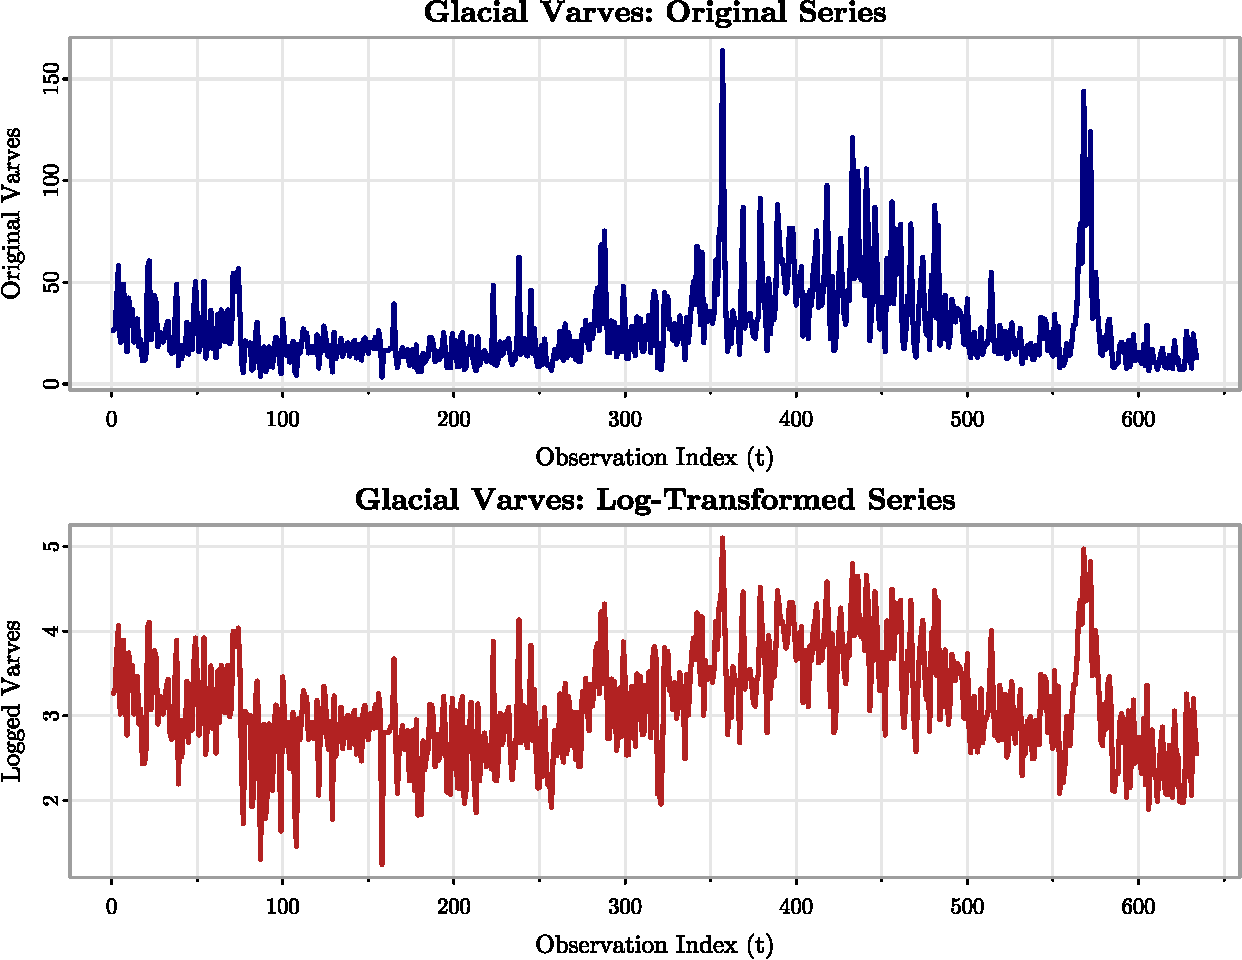
\includegraphics[width=\linewidth]{Homework6_files/figure-latex/p1a-timeplots-1} \end{center}

\begin{Shaded}
\begin{Highlighting}[]
\FunctionTok{with\_family}\NormalTok{(\{}
  \CommentTok{\# Compare marginal shape and normality before and after logging.}
\NormalTok{  op }\OtherTok{\textless{}{-}} \FunctionTok{par}\NormalTok{(}\AttributeTok{no.readonly =} \ConstantTok{TRUE}\NormalTok{)}
  \FunctionTok{on.exit}\NormalTok{(}\FunctionTok{par}\NormalTok{(op), }\AttributeTok{add =} \ConstantTok{TRUE}\NormalTok{)}
  \FunctionTok{par}\NormalTok{(}\AttributeTok{mfrow =} \FunctionTok{c}\NormalTok{(}\DecValTok{2}\NormalTok{, }\DecValTok{2}\NormalTok{), }\AttributeTok{mar =} \FunctionTok{c}\NormalTok{(}\FloatTok{4.2}\NormalTok{, }\FloatTok{4.5}\NormalTok{, }\FloatTok{2.8}\NormalTok{, }\FloatTok{1.2}\NormalTok{), }\AttributeTok{mgp =} \FunctionTok{c}\NormalTok{(}\FloatTok{2.2}\NormalTok{, }\FloatTok{0.7}\NormalTok{, }\DecValTok{0}\NormalTok{), }\AttributeTok{cex.main =} \FloatTok{1.05}\NormalTok{, }\AttributeTok{cex.lab =} \FloatTok{0.95}\NormalTok{, }\AttributeTok{cex.axis =} \FloatTok{0.9}\NormalTok{)}
  \FunctionTok{hist}\NormalTok{(varve\_x, }\AttributeTok{main =} \StringTok{\textquotesingle{}Histogram of Original Varves\textquotesingle{}}\NormalTok{, }\AttributeTok{xlab =} \StringTok{\textquotesingle{}Original Varves\textquotesingle{}}\NormalTok{, }\AttributeTok{col =} \StringTok{\textquotesingle{}gray85\textquotesingle{}}\NormalTok{, }\AttributeTok{border =} \StringTok{\textquotesingle{}gray40\textquotesingle{}}\NormalTok{)}
  \FunctionTok{qqnorm}\NormalTok{(varve\_x, }\AttributeTok{main =} \StringTok{\textquotesingle{}QQ Plot of Original Varves\textquotesingle{}}\NormalTok{, }\AttributeTok{pch =} \DecValTok{16}\NormalTok{, }\AttributeTok{cex =} \FloatTok{0.6}\NormalTok{, }\AttributeTok{col =} \StringTok{\textquotesingle{}navy\textquotesingle{}}\NormalTok{)}
  \FunctionTok{qqline}\NormalTok{(varve\_x, }\AttributeTok{col =} \StringTok{\textquotesingle{}firebrick\textquotesingle{}}\NormalTok{, }\AttributeTok{lwd =} \DecValTok{2}\NormalTok{)}
  \FunctionTok{hist}\NormalTok{(varve\_y, }\AttributeTok{main =} \StringTok{\textquotesingle{}Histogram of Logged Varves\textquotesingle{}}\NormalTok{, }\AttributeTok{xlab =} \StringTok{\textquotesingle{}Logged Varves\textquotesingle{}}\NormalTok{, }\AttributeTok{col =} \StringTok{\textquotesingle{}gray85\textquotesingle{}}\NormalTok{, }\AttributeTok{border =} \StringTok{\textquotesingle{}gray40\textquotesingle{}}\NormalTok{)}
  \FunctionTok{qqnorm}\NormalTok{(varve\_y, }\AttributeTok{main =} \StringTok{\textquotesingle{}QQ Plot of Logged Varves\textquotesingle{}}\NormalTok{, }\AttributeTok{pch =} \DecValTok{16}\NormalTok{, }\AttributeTok{cex =} \FloatTok{0.6}\NormalTok{, }\AttributeTok{col =} \StringTok{\textquotesingle{}navy\textquotesingle{}}\NormalTok{)}
  \FunctionTok{qqline}\NormalTok{(varve\_y, }\AttributeTok{col =} \StringTok{\textquotesingle{}firebrick\textquotesingle{}}\NormalTok{, }\AttributeTok{lwd =} \DecValTok{2}\NormalTok{)}
\NormalTok{\})}
\end{Highlighting}
\end{Shaded}

\begin{center}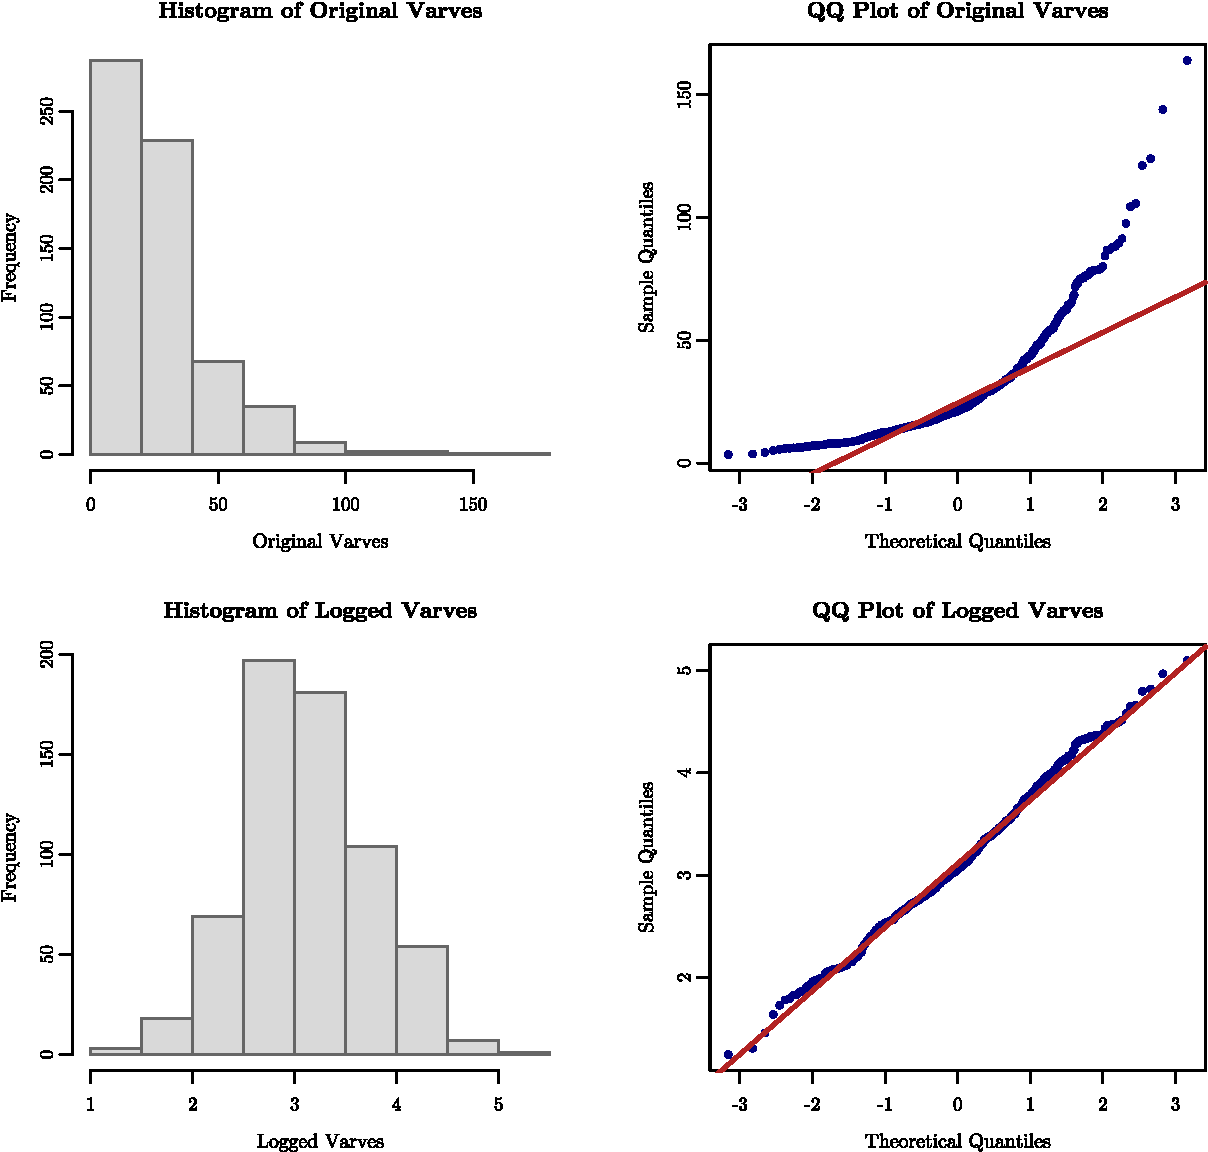
\includegraphics[width=\linewidth]{Homework6_files/figure-latex/p1a-hist-qq-1} \end{center}

The first-half and second-half sample variances for the original series are
\[
s^2_{X,\text{first}} = 133.4574
\quad \text{and} \quad
s^2_{X,\text{second}} = 594.4904.
\]
The second-half variance is about 4.4545 times the first-half variance, so the spread clearly increases over time. That is evidence of heteroscedasticity in \(X_t\). After the logarithmic transformation \(Y_t = \log(X_t)\), the first-half and second-half sample variances become
\[
s^2_{Y,\text{first}} = 0.2707
\quad \text{and} \quad
s^2_{Y,\text{second}} = 0.4514.
\]
Now the second-half variance is only about 1.6673 times the first-half variance, which is much closer to \(1\). So the log transformation stabilizes the variance substantially, even though it does not make the two halves exactly equal. From the plots:

\begin{itemize}
\tightlist
\item
  The time plot of \(X_t\) shows visibly wider fluctuations in the later portion of the record than in the earlier portion, whereas the time plot of \(Y_t\) compresses the larger values and reduces that widening.
\item
  The histogram of \(X_t\) is strongly right-skewed, and the QQ plot of \(X_t\) shows substantial deviation from a straight line, especially in the upper tail.
\item
  The histogram of \(Y_t\) is more symmetric than that of \(X_t\), and the QQ plot of \(Y_t\) is closer to linear, although there are still some tail departures.
\end{itemize}

Therefore, the log transformation improves both variance stability and the approximation to normality.

\newpage

\subsection{Problem 1 (b)}\label{problem-1-b}

\begin{problem}[Problem 1 (b)]
Make ACF of \(X_t\) and \(Y_t\) to compare them. Comment.
\end{problem}

\begin{Shaded}
\begin{Highlighting}[]
\CommentTok{\# Compute the ACFs for the original and logged series.}
\FunctionTok{acf}\NormalTok{(varve\_x, }\AttributeTok{plot =} \ConstantTok{FALSE}\NormalTok{, }\AttributeTok{lag.max =} \DecValTok{40}\NormalTok{)}
\FunctionTok{acf}\NormalTok{(varve\_y, }\AttributeTok{plot =} \ConstantTok{FALSE}\NormalTok{, }\AttributeTok{lag.max =} \DecValTok{40}\NormalTok{)}
\end{Highlighting}
\end{Shaded}

\begin{Shaded}
\begin{Highlighting}[]
\FunctionTok{with\_family}\NormalTok{(\{}
  \CommentTok{\# Plot the ACFs to compare persistence before and after logging.}
\NormalTok{  op }\OtherTok{\textless{}{-}} \FunctionTok{par}\NormalTok{(}\AttributeTok{no.readonly =} \ConstantTok{TRUE}\NormalTok{)}
  \FunctionTok{on.exit}\NormalTok{(}\FunctionTok{par}\NormalTok{(op), }\AttributeTok{add =} \ConstantTok{TRUE}\NormalTok{)}
  \FunctionTok{par}\NormalTok{(}\AttributeTok{mfrow =} \FunctionTok{c}\NormalTok{(}\DecValTok{2}\NormalTok{, }\DecValTok{1}\NormalTok{), }\AttributeTok{mar =} \FunctionTok{c}\NormalTok{(}\FloatTok{4.2}\NormalTok{, }\FloatTok{4.5}\NormalTok{, }\FloatTok{2.8}\NormalTok{, }\FloatTok{1.2}\NormalTok{), }\AttributeTok{mgp =} \FunctionTok{c}\NormalTok{(}\FloatTok{2.2}\NormalTok{, }\FloatTok{0.7}\NormalTok{, }\DecValTok{0}\NormalTok{), }\AttributeTok{cex.main =} \FloatTok{1.1}\NormalTok{, }\AttributeTok{cex.lab =} \DecValTok{1}\NormalTok{, }\AttributeTok{cex.axis =} \FloatTok{0.95}\NormalTok{)}
  \FunctionTok{acf}\NormalTok{(varve\_x, }\AttributeTok{lag.max =} \DecValTok{40}\NormalTok{, }\AttributeTok{main =} \StringTok{\textquotesingle{}ACF of Original Varves\textquotesingle{}}\NormalTok{, }\AttributeTok{col =} \StringTok{\textquotesingle{}navy\textquotesingle{}}\NormalTok{, }\AttributeTok{lwd =} \DecValTok{2}\NormalTok{)}
  \FunctionTok{acf}\NormalTok{(varve\_y, }\AttributeTok{lag.max =} \DecValTok{40}\NormalTok{, }\AttributeTok{main =} \StringTok{\textquotesingle{}ACF of Logged Varves\textquotesingle{}}\NormalTok{, }\AttributeTok{col =} \StringTok{\textquotesingle{}firebrick\textquotesingle{}}\NormalTok{, }\AttributeTok{lwd =} \DecValTok{2}\NormalTok{)}
\NormalTok{\})}
\end{Highlighting}
\end{Shaded}

\begin{center}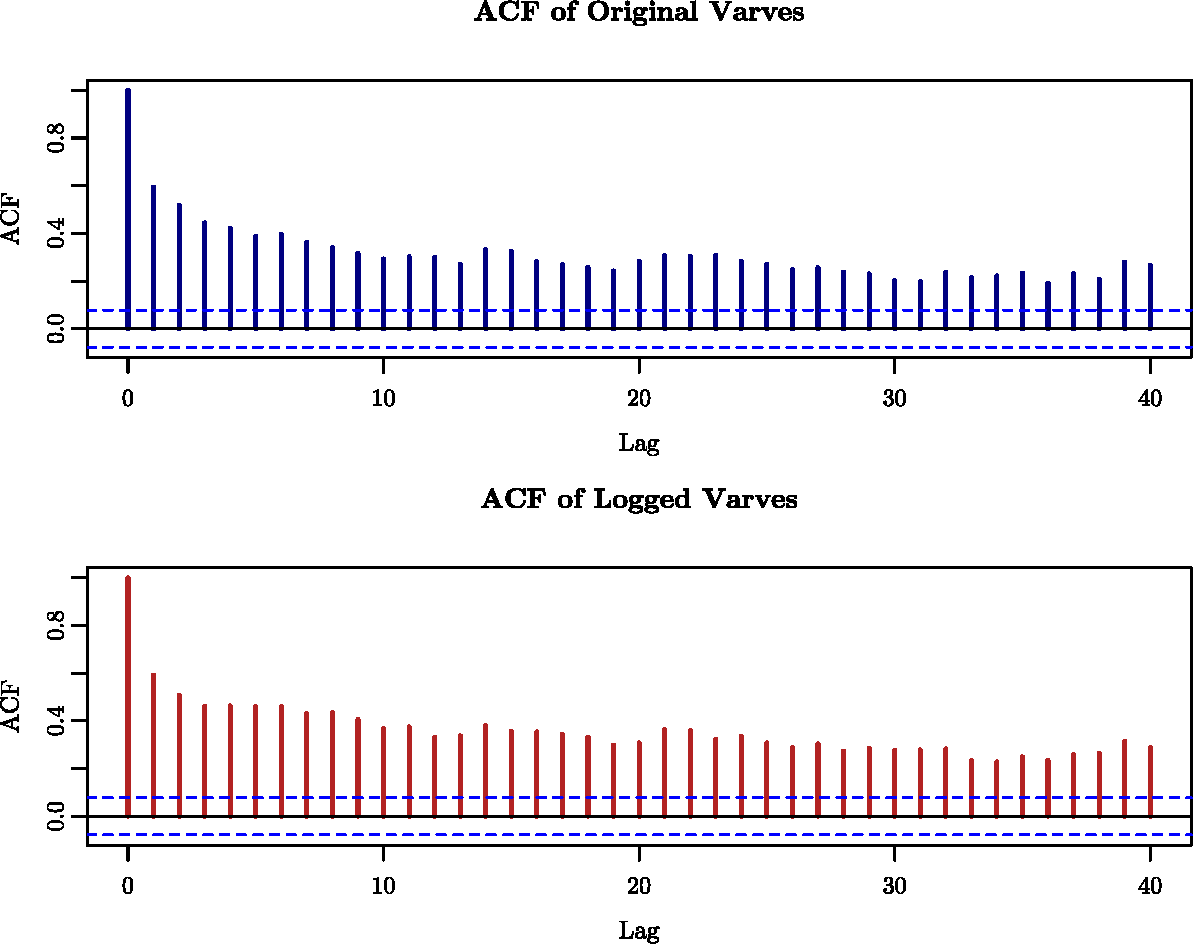
\includegraphics[width=\linewidth]{Homework6_files/figure-latex/p1b-acf-plot-1} \end{center}

The ACFs of \(X_t\) and \(Y_t\) are very similar in their overall shape. In both plots, many positive autocorrelations remain large across a long sequence of lags and decay only slowly instead of dropping off quickly toward \(0\). So the log transformation helps stabilize the variance, but it does not remove the strong serial dependence or the remaining non-stationarity in the mean behavior. The logged series is still too persistent to be treated as stationary.

\newpage

\subsection{Problem 1 (c)}\label{problem-1-c}

\begin{problem}[Problem 1 (c)]
Compute the difference of \(Y_t\) as \(U_t=Y_t-Y_{t-1}\), examine its time plot and sample ACF, and argue that differencing the logged varve data produces a reasonably stationary series.
\end{problem}

\begin{Shaded}
\begin{Highlighting}[]
\CommentTok{\# First{-}difference the logged varve series and inspect the first values.}
\NormalTok{varve\_u }\OtherTok{\textless{}{-}} \FunctionTok{diff}\NormalTok{(varve\_y)}
\FunctionTok{head}\NormalTok{(}\FunctionTok{data.frame}\NormalTok{(}
  \AttributeTok{t =} \DecValTok{2}\SpecialCharTok{:}\FunctionTok{length}\NormalTok{(varve\_y),}
  \AttributeTok{U\_t =}\NormalTok{ varve\_u}
\NormalTok{))}
\FunctionTok{acf}\NormalTok{(varve\_u, }\AttributeTok{plot =} \ConstantTok{FALSE}\NormalTok{, }\AttributeTok{lag.max =} \DecValTok{40}\NormalTok{)}
\end{Highlighting}
\end{Shaded}

\begin{Shaded}
\begin{Highlighting}[]
\FunctionTok{with\_family}\NormalTok{(\{}
  \CommentTok{\# Plot the differenced logged series and its sample ACF.}
\NormalTok{  op }\OtherTok{\textless{}{-}} \FunctionTok{par}\NormalTok{(}\AttributeTok{no.readonly =} \ConstantTok{TRUE}\NormalTok{)}
  \FunctionTok{on.exit}\NormalTok{(}\FunctionTok{par}\NormalTok{(op), }\AttributeTok{add =} \ConstantTok{TRUE}\NormalTok{)}
  \FunctionTok{par}\NormalTok{(}\AttributeTok{mfrow =} \FunctionTok{c}\NormalTok{(}\DecValTok{2}\NormalTok{, }\DecValTok{1}\NormalTok{), }\AttributeTok{mar =} \FunctionTok{c}\NormalTok{(}\FloatTok{4.2}\NormalTok{, }\FloatTok{4.5}\NormalTok{, }\FloatTok{2.8}\NormalTok{, }\FloatTok{1.2}\NormalTok{), }\AttributeTok{mgp =} \FunctionTok{c}\NormalTok{(}\FloatTok{2.2}\NormalTok{, }\FloatTok{0.7}\NormalTok{, }\DecValTok{0}\NormalTok{), }\AttributeTok{cex.main =} \FloatTok{1.1}\NormalTok{, }\AttributeTok{cex.lab =} \DecValTok{1}\NormalTok{, }\AttributeTok{cex.axis =} \FloatTok{0.95}\NormalTok{)}
\NormalTok{  astsa}\SpecialCharTok{::}\FunctionTok{tsplot}\NormalTok{(}
    \FunctionTok{ts}\NormalTok{(varve\_u, }\AttributeTok{start =} \DecValTok{2}\NormalTok{, }\AttributeTok{frequency =} \DecValTok{1}\NormalTok{),}
    \AttributeTok{main =} \StringTok{\textquotesingle{}Differenced Logged Varves\textquotesingle{}}\NormalTok{,}
    \AttributeTok{xlab =} \StringTok{\textquotesingle{}Observation Index (t)\textquotesingle{}}\NormalTok{,}
    \AttributeTok{ylab =} \StringTok{\textquotesingle{}U\_t\textquotesingle{}}\NormalTok{,}
    \AttributeTok{col =} \StringTok{\textquotesingle{}darkgreen\textquotesingle{}}\NormalTok{,}
    \AttributeTok{lwd =} \DecValTok{2}
\NormalTok{  )}
  \FunctionTok{acf}\NormalTok{(varve\_u, }\AttributeTok{lag.max =} \DecValTok{40}\NormalTok{, }\AttributeTok{main =} \StringTok{\textquotesingle{}Sample ACF of Differenced Logged Varves\textquotesingle{}}\NormalTok{, }\AttributeTok{col =} \StringTok{\textquotesingle{}darkgreen\textquotesingle{}}\NormalTok{, }\AttributeTok{lwd =} \DecValTok{2}\NormalTok{)}
\NormalTok{\})}
\end{Highlighting}
\end{Shaded}

\begin{center}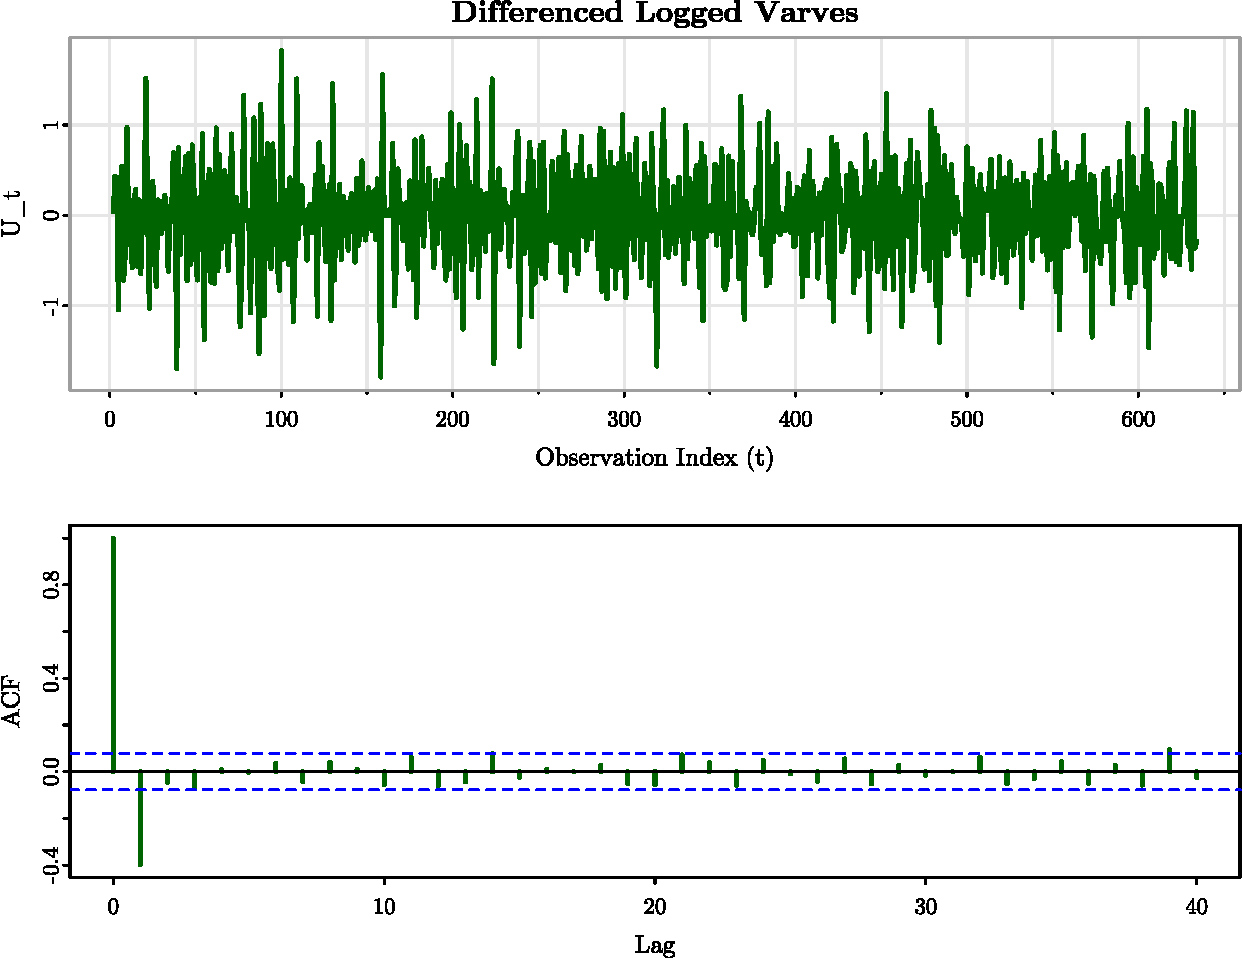
\includegraphics[width=\linewidth]{Homework6_files/figure-latex/p1c-plot-1} \end{center}

After first differencing the logged series,
\[
U_t = Y_t - Y_{t-1} = (1-B)Y_t.
\]
The differenced logged series fluctuates around a stable center near
\[
\bar U = -0.0011,
\]
and its spread looks much more stable than that of \(X_t\) or \(Y_t\). Its sample ACF also changes substantially. The main feature is that the very slow decay seen in \(X_t\) and \(Y_t\) is gone. After lag \(0\), there is one noticeable negative spike at lag \(1\), while the remaining autocorrelations are comparatively small and do not show a long persistent tail. Therefore, differencing the logged varve data removes the main low-frequency non-stationarity and produces a series that is reasonably stationary: its mean looks approximately constant over time, its variance is much more stable, and its sample ACF no longer shows the prolonged dependence seen in \(X_t\) and \(Y_t\).

\newpage

\section{Problem 2}\label{problem-2}

\begin{problem}[Problem 2]
Suppose that a time series \(X_t\) is transformed to another series \(Y_t\) as follows:
\[
Y_t = (1-B^{12})\log(X_t).
\]
Explain the mathematical steps in this transformation (see Lecture-12). Suggest a situation where this transformation would be useful.
\end{problem}

Let
\[
Z_t = \log(X_t).
\]
Then the given transformation becomes
\[
Y_t = (1-B^{12})Z_t.
\]

Since the backshift operator satisfies
\[
BZ_t = Z_{t-1},
\]
applying it \(12\) times gives
\[
B^{12}Z_t = Z_{t-12}.
\]
Therefore,
\[
\begin{aligned}
Y_t
&= (1-B^{12})Z_t \\
&= Z_t - B^{12}Z_t \\
&= Z_t - Z_{t-12} \\
&= \log(X_t) - \log(X_{t-12}) \\
&= \log\left(\frac{X_t}{X_{t-12}}\right).
\end{aligned}
\]

So this transformation has two steps:

\begin{enumerate}
\def\labelenumi{\arabic{enumi}.}
\item
  First, take logarithms:
  \[
  Z_t = \log(X_t).
  \]
  This is used for a positive-valued series when the spread tends to increase with the level.
\item
  Second, take a lag-12 difference:
  \[
  Y_t = Z_t - Z_{t-12}.
  \]
  This removes annual seasonality for monthly data, since lag \(12\) compares each month with the same month one year earlier. Hence, \(Y_t\) is the seasonal log-difference of \(X_t\), or equivalently the logarithm of the year-over-year ratio \(X_t / X_{t-12}\). This transformation is useful for a positive monthly time series that has both:
\end{enumerate}

\begin{itemize}
\tightlist
\item
  heteroscedasticity, so a logarithm is appropriate, and
\item
  seasonal behavior with period \(12\), so a seasonal difference is appropriate.
\end{itemize}

A standard example is monthly airline-passenger or monthly electricity-demand data, where the level and variance both increase over time and the same months tend to behave similarly from year to year.

\newpage

\section{Problem 3}\label{problem-3}

\begin{problem}[Problem 3]
For the \texttt{AirPassengers} data used for log transformation in Lecture 12, try the Box-Cox transformation to answer the following:
\end{problem}

\newpage

\subsection{Problem 3 (a)}\label{problem-3-a}

\begin{problem}[Problem 3 (a)]
What value of \(\lambda\) is selected?
\end{problem}

\begin{Shaded}
\begin{Highlighting}[]
\CommentTok{\# Compute the Box{-}Cox lambda selected by the data.}
\NormalTok{air\_lambda}
\end{Highlighting}
\end{Shaded}

\begin{verbatim}
## [1] -0.2947156
\end{verbatim}

Using \texttt{BoxCox.lambda(AirPassengers)}, the selected value is
\[
\hat{\lambda} = -0.2947.
\]

\newpage

\subsection{Problem 3 (b)}\label{problem-3-b}

\begin{problem}[Problem 3 (b)]
How does the transformed series compare to the log transformation?
\end{problem}

\begin{Shaded}
\begin{Highlighting}[]
\CommentTok{\# Compare first{-}half and second{-}half variances across three scales.}
\NormalTok{air\_lambda }\OtherTok{\textless{}{-}}\NormalTok{ forecast}\SpecialCharTok{::}\FunctionTok{BoxCox.lambda}\NormalTok{(AirPassengers)}
\NormalTok{air\_boxcox }\OtherTok{\textless{}{-}}\NormalTok{ forecast}\SpecialCharTok{::}\FunctionTok{BoxCox}\NormalTok{(AirPassengers, }\AttributeTok{lambda =}\NormalTok{ air\_lambda)}
\FunctionTok{data.frame}\NormalTok{(}
  \AttributeTok{Scale =} \FunctionTok{c}\NormalTok{(}\StringTok{\textquotesingle{}Original\textquotesingle{}}\NormalTok{, }\StringTok{\textquotesingle{}Log\textquotesingle{}}\NormalTok{, }\StringTok{\textquotesingle{}Box{-}Cox\textquotesingle{}}\NormalTok{),}
  \AttributeTok{First\_Half =} \FunctionTok{c}\NormalTok{(}
    \FunctionTok{var}\NormalTok{(}\FunctionTok{as.numeric}\NormalTok{(air\_x)[}\DecValTok{1}\SpecialCharTok{:}\DecValTok{72}\NormalTok{]),}
    \FunctionTok{var}\NormalTok{(}\FunctionTok{as.numeric}\NormalTok{(air\_log)[}\DecValTok{1}\SpecialCharTok{:}\DecValTok{72}\NormalTok{]),}
    \FunctionTok{var}\NormalTok{(}\FunctionTok{as.numeric}\NormalTok{(air\_boxcox)[}\DecValTok{1}\SpecialCharTok{:}\DecValTok{72}\NormalTok{])}
\NormalTok{  ),}
  \AttributeTok{Second\_Half =} \FunctionTok{c}\NormalTok{(}
    \FunctionTok{var}\NormalTok{(}\FunctionTok{as.numeric}\NormalTok{(air\_x)[}\DecValTok{73}\SpecialCharTok{:}\DecValTok{144}\NormalTok{]),}
    \FunctionTok{var}\NormalTok{(}\FunctionTok{as.numeric}\NormalTok{(air\_log)[}\DecValTok{73}\SpecialCharTok{:}\DecValTok{144}\NormalTok{]),}
    \FunctionTok{var}\NormalTok{(}\FunctionTok{as.numeric}\NormalTok{(air\_boxcox)[}\DecValTok{73}\SpecialCharTok{:}\DecValTok{144}\NormalTok{])}
\NormalTok{  )}
\NormalTok{)}
\end{Highlighting}
\end{Shaded}

\begin{Shaded}
\begin{Highlighting}[]
\FunctionTok{with\_family}\NormalTok{(\{}
  \CommentTok{\# Plot the original, log{-}transformed, and Box{-}Cox{-}transformed series.}
\NormalTok{  op }\OtherTok{\textless{}{-}} \FunctionTok{par}\NormalTok{(}\AttributeTok{no.readonly =} \ConstantTok{TRUE}\NormalTok{)}
  \FunctionTok{on.exit}\NormalTok{(}\FunctionTok{par}\NormalTok{(op), }\AttributeTok{add =} \ConstantTok{TRUE}\NormalTok{)}
  \FunctionTok{par}\NormalTok{(}\AttributeTok{mfrow =} \FunctionTok{c}\NormalTok{(}\DecValTok{3}\NormalTok{, }\DecValTok{1}\NormalTok{), }\AttributeTok{mar =} \FunctionTok{c}\NormalTok{(}\FloatTok{4.2}\NormalTok{, }\FloatTok{4.5}\NormalTok{, }\FloatTok{2.8}\NormalTok{, }\FloatTok{1.2}\NormalTok{), }\AttributeTok{mgp =} \FunctionTok{c}\NormalTok{(}\FloatTok{2.2}\NormalTok{, }\FloatTok{0.7}\NormalTok{, }\DecValTok{0}\NormalTok{), }\AttributeTok{cex.main =} \FloatTok{1.05}\NormalTok{, }\AttributeTok{cex.lab =} \FloatTok{0.95}\NormalTok{, }\AttributeTok{cex.axis =} \FloatTok{0.9}\NormalTok{)}
\NormalTok{  astsa}\SpecialCharTok{::}\FunctionTok{tsplot}\NormalTok{(air\_x, }\AttributeTok{main =} \StringTok{\textquotesingle{}AirPassengers: Original Series\textquotesingle{}}\NormalTok{, }\AttributeTok{xlab =} \StringTok{\textquotesingle{}Time (Months)\textquotesingle{}}\NormalTok{, }\AttributeTok{ylab =} \StringTok{\textquotesingle{}Passengers\textquotesingle{}}\NormalTok{, }\AttributeTok{col =} \StringTok{\textquotesingle{}navy\textquotesingle{}}\NormalTok{, }\AttributeTok{lwd =} \DecValTok{2}\NormalTok{)}
\NormalTok{  astsa}\SpecialCharTok{::}\FunctionTok{tsplot}\NormalTok{(air\_log, }\AttributeTok{main =} \StringTok{\textquotesingle{}AirPassengers: Log Transformation\textquotesingle{}}\NormalTok{, }\AttributeTok{xlab =} \StringTok{\textquotesingle{}Time (Months)\textquotesingle{}}\NormalTok{, }\AttributeTok{ylab =} \StringTok{\textquotesingle{}log(Passengers)\textquotesingle{}}\NormalTok{, }\AttributeTok{col =} \StringTok{\textquotesingle{}firebrick\textquotesingle{}}\NormalTok{, }\AttributeTok{lwd =} \DecValTok{2}\NormalTok{)}
\NormalTok{  astsa}\SpecialCharTok{::}\FunctionTok{tsplot}\NormalTok{(air\_boxcox, }\AttributeTok{main =} \FunctionTok{paste0}\NormalTok{(}\StringTok{\textquotesingle{}AirPassengers: Box{-}Cox Transformation (lambda = \textquotesingle{}}\NormalTok{, }\FunctionTok{round}\NormalTok{(air\_lambda, }\DecValTok{4}\NormalTok{), }\StringTok{\textquotesingle{})\textquotesingle{}}\NormalTok{), }\AttributeTok{xlab =} \StringTok{\textquotesingle{}Time (Months)\textquotesingle{}}\NormalTok{, }\AttributeTok{ylab =} \StringTok{\textquotesingle{}Box{-}Cox Scale\textquotesingle{}}\NormalTok{, }\AttributeTok{col =} \StringTok{\textquotesingle{}darkgreen\textquotesingle{}}\NormalTok{, }\AttributeTok{lwd =} \DecValTok{2}\NormalTok{)}
\NormalTok{\})}
\end{Highlighting}
\end{Shaded}

\begin{center}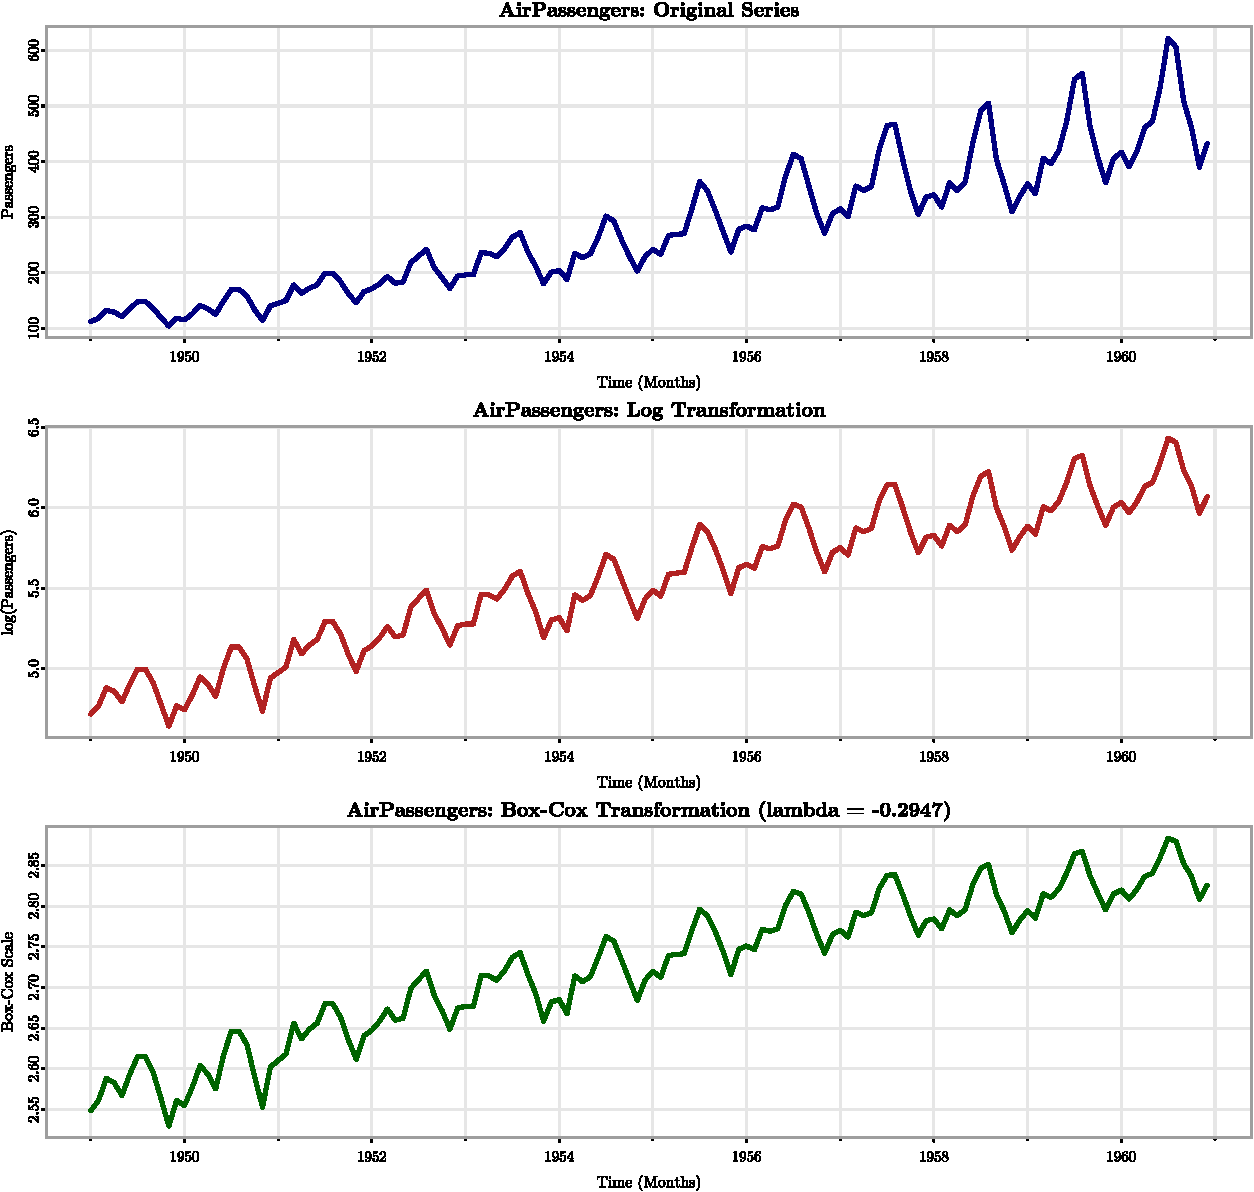
\includegraphics[width=\linewidth]{Homework6_files/figure-latex/p3b-plot-1} \end{center}

\begin{center}
\small
\begin{table}[H]

\caption{\label{tab:p3b-var-table}First-half and second-half sample variances for the AirPassengers series under different scales}
\centering
\begin{tabular}[t]{cccc}
\toprule
Scale & First Half Variance & Second Half Variance & Second/First Ratio\\
\midrule
Original & 2275.6946 & 7471.7363 & 3.2833\\
Log & 0.0693 & 0.0500 & 0.7205\\
Box-Cox ($\lambda=-0.2947$) & 0.0033 & 0.0015 & 0.4598\\
\bottomrule
\end{tabular}
\end{table}
\normalsize
\end{center}

Because \(\hat{\lambda} = -0.2947\) is reasonably close to \(0\), the Box-Cox transformed series is broadly similar to the log-transformed series. Both transformations compress the larger passenger counts in the later years and reduce the visible fanning-out that appears in the original series. However, since \(\hat{\lambda}<0\), the Box-Cox transformation compresses the larger observations slightly more strongly than the log transformation. So, relative to \(\log(X_t)\), the Box-Cox series has a somewhat flatter upper end in the later part of the record.

\newpage

\subsection{Problem 3 (c)}\label{problem-3-c}

\begin{problem}[Problem 3 (c)]
Does variance appear stabilized?
\end{problem}

Yes, the variance appears stabilized after the Box-Cox transformation. In the original series, the second-half variance is
\[
3.2833
\]
times the first-half variance, which shows substantial increase in spread over time. After the log transformation, that ratio becomes
\[
0.7205,
\]
and after the Box-Cox transformation it becomes
\[
0.4598.
\]

So both log and Box-Cox stabilize the variance substantially relative to the original scale. Visually, the Box-Cox series does look variance-stabilized, although in this case the log transformation already does most of that work and the Box-Cox result is not dramatically different from it.

\newpage

\section{Problem 4}\label{problem-4}

\begin{problem}[Problem 4]
Consider the \texttt{EuStockMarkets} data in \textsf{R}. For this problem, I use the DAX series.
\end{problem}

\newpage

\subsection{Problem 4 (a)}\label{problem-4-a}

\begin{problem}[Problem 4 (a)]
Plot the time series for DAX. Is it stationary?
\end{problem}

\begin{Shaded}
\begin{Highlighting}[]
\CommentTok{\# Display the first few DAX observations.}
\FunctionTok{head}\NormalTok{(}\FunctionTok{data.frame}\NormalTok{(}
  \AttributeTok{t =} \FunctionTok{seq\_along}\NormalTok{(dax),}
  \AttributeTok{DAX =}\NormalTok{ dax}
\NormalTok{))}
\end{Highlighting}
\end{Shaded}

\begin{Shaded}
\begin{Highlighting}[]
\FunctionTok{with\_family}\NormalTok{(\{}
  \CommentTok{\# Plot the DAX level series.}
\NormalTok{  op }\OtherTok{\textless{}{-}} \FunctionTok{par}\NormalTok{(}\AttributeTok{no.readonly =} \ConstantTok{TRUE}\NormalTok{)}
  \FunctionTok{on.exit}\NormalTok{(}\FunctionTok{par}\NormalTok{(op), }\AttributeTok{add =} \ConstantTok{TRUE}\NormalTok{)}
  \FunctionTok{par}\NormalTok{(}\AttributeTok{mfrow =} \FunctionTok{c}\NormalTok{(}\DecValTok{1}\NormalTok{, }\DecValTok{1}\NormalTok{), }\AttributeTok{mar =} \FunctionTok{c}\NormalTok{(}\FloatTok{4.2}\NormalTok{, }\FloatTok{4.5}\NormalTok{, }\FloatTok{2.8}\NormalTok{, }\FloatTok{1.2}\NormalTok{), }\AttributeTok{mgp =} \FunctionTok{c}\NormalTok{(}\FloatTok{2.2}\NormalTok{, }\FloatTok{0.7}\NormalTok{, }\DecValTok{0}\NormalTok{), }\AttributeTok{cex.main =} \FloatTok{1.1}\NormalTok{, }\AttributeTok{cex.lab =} \DecValTok{1}\NormalTok{, }\AttributeTok{cex.axis =} \FloatTok{0.95}\NormalTok{)}
\NormalTok{  astsa}\SpecialCharTok{::}\FunctionTok{tsplot}\NormalTok{(}
\NormalTok{    dax\_ts,}
    \AttributeTok{main =} \StringTok{\textquotesingle{}DAX Index\textquotesingle{}}\NormalTok{,}
    \AttributeTok{xlab =} \StringTok{\textquotesingle{}Time\textquotesingle{}}\NormalTok{,}
    \AttributeTok{ylab =} \StringTok{\textquotesingle{}DAX Index Points\textquotesingle{}}\NormalTok{,}
    \AttributeTok{col =} \StringTok{\textquotesingle{}navy\textquotesingle{}}\NormalTok{,}
    \AttributeTok{lwd =} \DecValTok{2}
\NormalTok{  )}
\NormalTok{\})}
\end{Highlighting}
\end{Shaded}

\begin{center}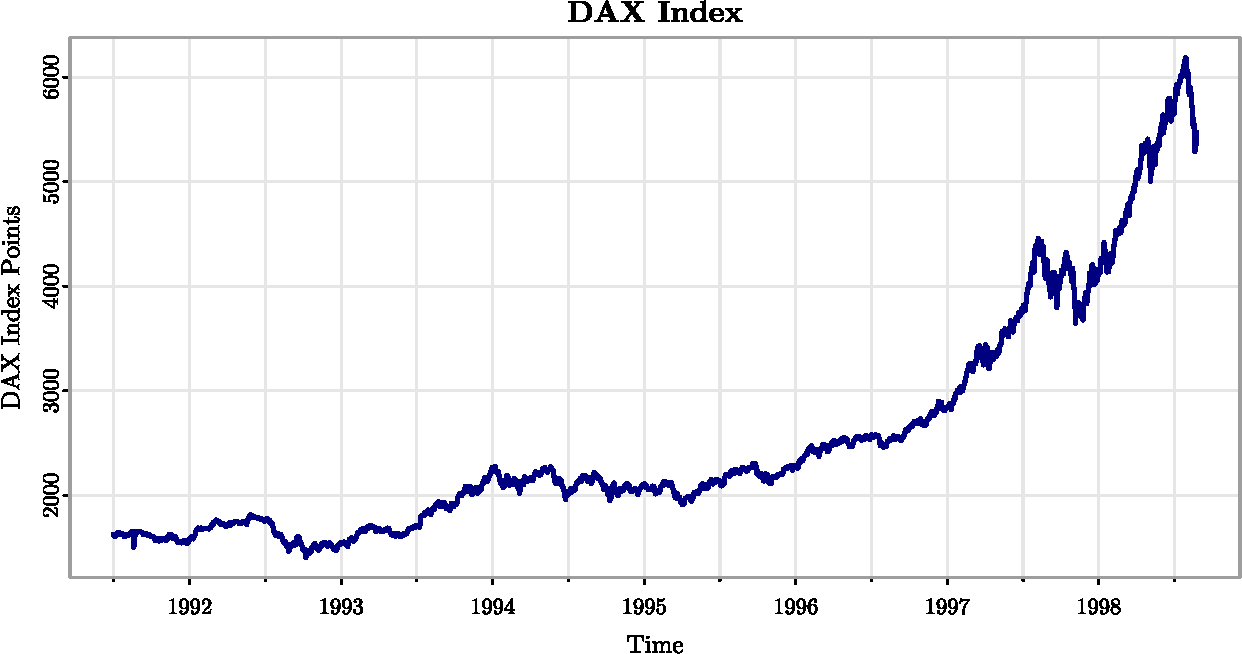
\includegraphics[width=\linewidth]{Homework6_files/figure-latex/p4a-plot-1} \end{center}

The data are daily DAX index levels over 1860 observations, measured in index points. The plot shows a strong upward long-run movement, so the mean is clearly not constant over time. The movement is not linear; the series rises unevenly, with both local accelerations and local pullbacks. There is no simple repeated seasonal pattern visible in the level plot. The spread is much larger in the later part of the series than in the earlier part, so the series also appears heteroscedastic. The statistical range is 1402.34 to 6186.09, so the total range is 4783.75 index points. No volatility. Since the mean and variance behavior both change over time, the DAX level series does not satisfy stationarity.

\newpage

\subsection{Problem 4 (b)}\label{problem-4-b}

\begin{problem}[Problem 4 (b)]
Plot the log returns of the DAX. How does it differ from the original series?
\end{problem}

For the log returns, I use
\[
R_t = \log(X_t)-\log(X_{t-1}) = (1-B)\log(X_t).
\]

\begin{Shaded}
\begin{Highlighting}[]
\CommentTok{\# Build the DAX log{-}return series.}
\NormalTok{dax\_log\_return }\OtherTok{\textless{}{-}} \FunctionTok{diff}\NormalTok{(}\FunctionTok{log}\NormalTok{(dax))}
\FunctionTok{head}\NormalTok{(}\FunctionTok{data.frame}\NormalTok{(}
  \AttributeTok{t =} \DecValTok{2}\SpecialCharTok{:}\FunctionTok{length}\NormalTok{(dax),}
  \AttributeTok{Log\_Return =}\NormalTok{ dax\_log\_return}
\NormalTok{))}
\end{Highlighting}
\end{Shaded}

\begin{Shaded}
\begin{Highlighting}[]
\FunctionTok{with\_family}\NormalTok{(\{}
  \CommentTok{\# Plot the DAX log returns.}
\NormalTok{  op }\OtherTok{\textless{}{-}} \FunctionTok{par}\NormalTok{(}\AttributeTok{no.readonly =} \ConstantTok{TRUE}\NormalTok{)}
  \FunctionTok{on.exit}\NormalTok{(}\FunctionTok{par}\NormalTok{(op), }\AttributeTok{add =} \ConstantTok{TRUE}\NormalTok{)}
  \FunctionTok{par}\NormalTok{(}\AttributeTok{mfrow =} \FunctionTok{c}\NormalTok{(}\DecValTok{1}\NormalTok{, }\DecValTok{1}\NormalTok{), }\AttributeTok{mar =} \FunctionTok{c}\NormalTok{(}\FloatTok{4.2}\NormalTok{, }\FloatTok{4.5}\NormalTok{, }\FloatTok{2.8}\NormalTok{, }\FloatTok{1.2}\NormalTok{), }\AttributeTok{mgp =} \FunctionTok{c}\NormalTok{(}\FloatTok{2.2}\NormalTok{, }\FloatTok{0.7}\NormalTok{, }\DecValTok{0}\NormalTok{), }\AttributeTok{cex.main =} \FloatTok{1.1}\NormalTok{, }\AttributeTok{cex.lab =} \DecValTok{1}\NormalTok{, }\AttributeTok{cex.axis =} \FloatTok{0.95}\NormalTok{)}
\NormalTok{  astsa}\SpecialCharTok{::}\FunctionTok{tsplot}\NormalTok{(}
\NormalTok{    stats}\SpecialCharTok{::}\FunctionTok{ts}\NormalTok{(dax\_log\_return, }\AttributeTok{start =} \DecValTok{2}\NormalTok{, }\AttributeTok{frequency =} \DecValTok{260}\NormalTok{),}
    \AttributeTok{main =} \StringTok{\textquotesingle{}DAX Log Returns\textquotesingle{}}\NormalTok{,}
    \AttributeTok{xlab =} \StringTok{\textquotesingle{}Time\textquotesingle{}}\NormalTok{,}
    \AttributeTok{ylab =} \StringTok{\textquotesingle{}Log Return\textquotesingle{}}\NormalTok{,}
    \AttributeTok{col =} \StringTok{\textquotesingle{}firebrick\textquotesingle{}}\NormalTok{,}
    \AttributeTok{lwd =} \DecValTok{2}
\NormalTok{  )}
\NormalTok{\})}
\end{Highlighting}
\end{Shaded}

\begin{center}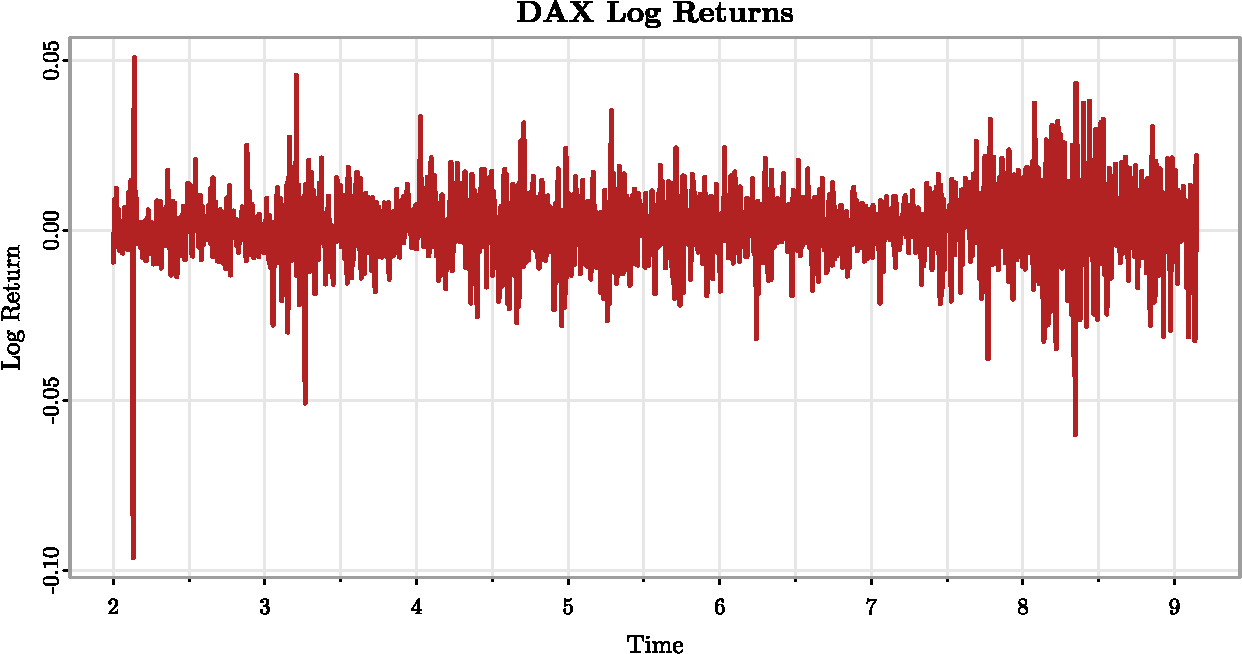
\includegraphics[width=\linewidth]{Homework6_files/figure-latex/p4b-plot-1} \end{center}

Compared with the original DAX level series, the log-return series is very different. Specifically, the log returns fluctuate around a center near 0.000652 rather than following a strong upward path. There is no visible deterministic trend in the log returns. The range is much smaller: from -0.0963 to 0.0508. The spread is much more stable than in the original level series, although there are still some clusters of larger and smaller movements, which is typical in financial-return data. No volatility still. Overall, the log-return series looks much more like short-run noise around a constant mean than the original series does.

\newpage

\subsection{Problem 4 (c)}\label{problem-4-c}

\begin{problem}[Problem 4 (c)]
Does the series appear more stationary after taking log returns? Justify.
\end{problem}

Yes, the series appears much more stationary after taking log returns. As I describe in the earlier part, the strong trend in the mean is removed and the variance is much more stable than on the original scale. Therefore, while the log-return series is not guaranteed to be perfectly stationary in every sense, but it appears much \emph{more} stationary than the original DAX level series and is far closer to a stationary time series.

\newpage

\section{Problem 5}\label{problem-5}

\begin{problem}[Problem 5]
For your data analysis project, does your detrended and deseasonalized data (both response and all predictors) need any transformations? Justify. Show the transformations and how they work for your variables.
\end{problem}

From Homework 5, \(G_t\) denotes the game-by-game even-strength GSAx response, measured in goals, at aligned game index \(t\). The predictor \(S_t\) denotes the game-by-game even-strength save percentage, recorded as a proportion, and \(X_t\) denotes the game-by-game team even-strength xGF\%, recorded in percentage points. The final Homework 5 lagged regression models used \(S_{t-4}\), \(X_{t-8}\), and \(G_{t-4}\) for Blackwood, and \(S_{t-2}\), \(X_{t-4}\), and \(G_{t-2}\) for Shesterkin. So, in this homework, the response series are already detrended and deseasonalized because I use the residuals from those final lagged regression models. The question is whether those residual response series, together with the aligned predictor series carried into the final models, still show enough heteroscedasticity to require an additional variance-stabilizing transformation. To do this, I will do the following:

\begin{enumerate}
\def\labelenumi{\arabic{enumi}.}
\tightlist
\item
  Check the detrended and deseasonalized series for visible fanning-out or a clear increase in spread over time.
\item
  Compare first-half and second-half sample variances (as we did in this homework; not really sure if this is a standard convention or not)
\item
  If the spread still increases enough to justify transformation, then compare candidate shifted log and shifted Box-Cox versions.
\item
  If not, keep the existing scale and only mean-correct.
\end{enumerate}

So the detrended and deseasonalized response series are
\[
\widehat{\varepsilon}^{(B)}_t = G_t - \widehat{G_t}^{(B)}
\quad \text{and} \quad
\widehat{\varepsilon}^{(S)}_t = G_t - \widehat{G_t}^{(S)}.
\]
Here, \(\widehat{G_t}^{(B)}\) and \(\widehat{G_t}^{(S)}\) are the fitted values from the final Homework 5 lagged regression models for Blackwood and Shesterkin, respectively.

\begin{Shaded}
\begin{Highlighting}[]
\CommentTok{\# Rebuild the final Homework 5 lagged regression models.}
\NormalTok{blackwood\_hw5 }\OtherTok{\textless{}{-}} \FunctionTok{build\_lagged\_regression\_hw5}\NormalTok{(blackwood\_gbgs, }\AttributeTok{sv\_lead =} \DecValTok{4}\NormalTok{, }\AttributeTok{x\_lead =} \DecValTok{8}\NormalTok{, }\AttributeTok{g\_lead =} \DecValTok{4}\NormalTok{)}
\NormalTok{shesterkin\_hw5 }\OtherTok{\textless{}{-}} \FunctionTok{build\_lagged\_regression\_hw5}\NormalTok{(shesterkin\_gbgs, }\AttributeTok{sv\_lead =} \DecValTok{2}\NormalTok{, }\AttributeTok{x\_lead =} \DecValTok{4}\NormalTok{, }\AttributeTok{g\_lead =} \DecValTok{2}\NormalTok{)}

\CommentTok{\# Extract the detrended and deseasonalized response series.}
\NormalTok{blackwood\_resid }\OtherTok{\textless{}{-}}\NormalTok{ stats}\SpecialCharTok{::}\FunctionTok{residuals}\NormalTok{(blackwood\_hw5}\SpecialCharTok{$}\NormalTok{fit)}
\NormalTok{shesterkin\_resid }\OtherTok{\textless{}{-}}\NormalTok{ stats}\SpecialCharTok{::}\FunctionTok{residuals}\NormalTok{(shesterkin\_hw5}\SpecialCharTok{$}\NormalTok{fit)}

\CommentTok{\# Build mean{-}only corrections for the already{-}detrended response series.}
\NormalTok{blackwood\_mean\_fit }\OtherTok{\textless{}{-}}\NormalTok{ stats}\SpecialCharTok{::}\FunctionTok{lm}\NormalTok{(blackwood\_resid }\SpecialCharTok{\textasciitilde{}} \DecValTok{1}\NormalTok{)}
\NormalTok{shesterkin\_mean\_fit }\OtherTok{\textless{}{-}}\NormalTok{ stats}\SpecialCharTok{::}\FunctionTok{lm}\NormalTok{(shesterkin\_resid }\SpecialCharTok{\textasciitilde{}} \DecValTok{1}\NormalTok{)}

\CommentTok{\# Helper to summarize variance balance before and after shifted log/Box{-}Cox transforms.}
\NormalTok{shifted\_transform\_review }\OtherTok{\textless{}{-}} \ControlFlowTok{function}\NormalTok{(z, label) \{}
\NormalTok{  n }\OtherTok{\textless{}{-}} \FunctionTok{length}\NormalTok{(z)}
\NormalTok{  h }\OtherTok{\textless{}{-}} \FunctionTok{floor}\NormalTok{(n }\SpecialCharTok{/} \DecValTok{2}\NormalTok{)}
\NormalTok{  shift\_c }\OtherTok{\textless{}{-}} \ControlFlowTok{if}\NormalTok{ (}\FunctionTok{min}\NormalTok{(z) }\SpecialCharTok{\textless{}=} \DecValTok{0}\NormalTok{) }\FunctionTok{abs}\NormalTok{(}\FunctionTok{min}\NormalTok{(z)) }\SpecialCharTok{+} \DecValTok{1} \ControlFlowTok{else} \DecValTok{0}
\NormalTok{  z\_shift }\OtherTok{\textless{}{-}}\NormalTok{ z }\SpecialCharTok{+}\NormalTok{ shift\_c}
\NormalTok{  lambda\_hat }\OtherTok{\textless{}{-}}\NormalTok{ forecast}\SpecialCharTok{::}\FunctionTok{BoxCox.lambda}\NormalTok{(z\_shift)}
\NormalTok{  z\_log }\OtherTok{\textless{}{-}} \FunctionTok{log}\NormalTok{(z\_shift)}
\NormalTok{  z\_bc }\OtherTok{\textless{}{-}}\NormalTok{ forecast}\SpecialCharTok{::}\FunctionTok{BoxCox}\NormalTok{(z\_shift, }\AttributeTok{lambda =}\NormalTok{ lambda\_hat)}
  \FunctionTok{data.frame}\NormalTok{(}
    \AttributeTok{Series =}\NormalTok{ label,}
    \AttributeTok{Shift =}\NormalTok{ shift\_c,}
    \AttributeTok{Lambda =}\NormalTok{ lambda\_hat,}
    \AttributeTok{Raw\_Ratio =}\NormalTok{ stats}\SpecialCharTok{::}\FunctionTok{var}\NormalTok{(z[(h }\SpecialCharTok{+} \DecValTok{1}\NormalTok{)}\SpecialCharTok{:}\NormalTok{n]) }\SpecialCharTok{/}\NormalTok{ stats}\SpecialCharTok{::}\FunctionTok{var}\NormalTok{(z[}\DecValTok{1}\SpecialCharTok{:}\NormalTok{h]),}
    \AttributeTok{Shifted\_Log\_Ratio =}\NormalTok{ stats}\SpecialCharTok{::}\FunctionTok{var}\NormalTok{(z\_log[(h }\SpecialCharTok{+} \DecValTok{1}\NormalTok{)}\SpecialCharTok{:}\NormalTok{n]) }\SpecialCharTok{/}\NormalTok{ stats}\SpecialCharTok{::}\FunctionTok{var}\NormalTok{(z\_log[}\DecValTok{1}\SpecialCharTok{:}\NormalTok{h]),}
    \AttributeTok{Shifted\_BoxCox\_Ratio =}\NormalTok{ stats}\SpecialCharTok{::}\FunctionTok{var}\NormalTok{(z\_bc[(h }\SpecialCharTok{+} \DecValTok{1}\NormalTok{)}\SpecialCharTok{:}\NormalTok{n]) }\SpecialCharTok{/}\NormalTok{ stats}\SpecialCharTok{::}\FunctionTok{var}\NormalTok{(z\_bc[}\DecValTok{1}\SpecialCharTok{:}\NormalTok{h]),}
    \AttributeTok{stringsAsFactors =} \ConstantTok{FALSE}
\NormalTok{  )}
\NormalTok{\}}

\CommentTok{\# Build project{-}specific diagnostic tables from the aligned series actually used in Homework 5.}
\NormalTok{blackwood\_diag\_table }\OtherTok{\textless{}{-}} \FunctionTok{rbind}\NormalTok{(}
  \FunctionTok{split\_variance\_table}\NormalTok{(blackwood\_resid, }\StringTok{\textquotesingle{}$}\SpecialCharTok{\textbackslash{}\textbackslash{}}\StringTok{widehat\{}\SpecialCharTok{\textbackslash{}\textbackslash{}}\StringTok{varepsilon\}\^{}\{(B)\}\_t$\textquotesingle{}}\NormalTok{),}
  \FunctionTok{split\_variance\_table}\NormalTok{(blackwood\_hw5}\SpecialCharTok{$}\NormalTok{data}\SpecialCharTok{$}\NormalTok{sv, }\StringTok{\textquotesingle{}$S\_\{t{-}4\}$\textquotesingle{}}\NormalTok{),}
  \FunctionTok{split\_variance\_table}\NormalTok{(blackwood\_hw5}\SpecialCharTok{$}\NormalTok{data}\SpecialCharTok{$}\NormalTok{xgf, }\StringTok{\textquotesingle{}$X\_\{t{-}8\}$\textquotesingle{}}\NormalTok{),}
  \FunctionTok{split\_variance\_table}\NormalTok{(blackwood\_hw5}\SpecialCharTok{$}\NormalTok{data}\SpecialCharTok{$}\NormalTok{gLag, }\StringTok{\textquotesingle{}$G\_\{t{-}4\}$\textquotesingle{}}\NormalTok{)}
\NormalTok{)}
\NormalTok{blackwood\_diag\_table}\SpecialCharTok{$}\NormalTok{Mean }\OtherTok{\textless{}{-}} \FunctionTok{c}\NormalTok{(}
  \FunctionTok{mean}\NormalTok{(blackwood\_resid),}
  \FunctionTok{mean}\NormalTok{(blackwood\_hw5}\SpecialCharTok{$}\NormalTok{data}\SpecialCharTok{$}\NormalTok{sv),}
  \FunctionTok{mean}\NormalTok{(blackwood\_hw5}\SpecialCharTok{$}\NormalTok{data}\SpecialCharTok{$}\NormalTok{xgf),}
  \FunctionTok{mean}\NormalTok{(blackwood\_hw5}\SpecialCharTok{$}\NormalTok{data}\SpecialCharTok{$}\NormalTok{gLag)}
\NormalTok{)}
\NormalTok{blackwood\_diag\_table}\SpecialCharTok{$}\NormalTok{Min }\OtherTok{\textless{}{-}} \FunctionTok{c}\NormalTok{(}
  \FunctionTok{min}\NormalTok{(blackwood\_resid),}
  \FunctionTok{min}\NormalTok{(blackwood\_hw5}\SpecialCharTok{$}\NormalTok{data}\SpecialCharTok{$}\NormalTok{sv),}
  \FunctionTok{min}\NormalTok{(blackwood\_hw5}\SpecialCharTok{$}\NormalTok{data}\SpecialCharTok{$}\NormalTok{xgf),}
  \FunctionTok{min}\NormalTok{(blackwood\_hw5}\SpecialCharTok{$}\NormalTok{data}\SpecialCharTok{$}\NormalTok{gLag)}
\NormalTok{)}
\NormalTok{blackwood\_diag\_table}\SpecialCharTok{$}\NormalTok{Max }\OtherTok{\textless{}{-}} \FunctionTok{c}\NormalTok{(}
  \FunctionTok{max}\NormalTok{(blackwood\_resid),}
  \FunctionTok{max}\NormalTok{(blackwood\_hw5}\SpecialCharTok{$}\NormalTok{data}\SpecialCharTok{$}\NormalTok{sv),}
  \FunctionTok{max}\NormalTok{(blackwood\_hw5}\SpecialCharTok{$}\NormalTok{data}\SpecialCharTok{$}\NormalTok{xgf),}
  \FunctionTok{max}\NormalTok{(blackwood\_hw5}\SpecialCharTok{$}\NormalTok{data}\SpecialCharTok{$}\NormalTok{gLag)}
\NormalTok{)}
\NormalTok{blackwood\_diag\_table }\OtherTok{\textless{}{-}}\NormalTok{ blackwood\_diag\_table[, }\FunctionTok{c}\NormalTok{(}\StringTok{\textquotesingle{}Series\textquotesingle{}}\NormalTok{, }\StringTok{\textquotesingle{}Mean\textquotesingle{}}\NormalTok{, }\StringTok{\textquotesingle{}Min\textquotesingle{}}\NormalTok{, }\StringTok{\textquotesingle{}Max\textquotesingle{}}\NormalTok{, }\StringTok{\textquotesingle{}First\_Half\textquotesingle{}}\NormalTok{, }\StringTok{\textquotesingle{}Second\_Half\textquotesingle{}}\NormalTok{, }\StringTok{\textquotesingle{}Ratio\_Second\_to\_First\textquotesingle{}}\NormalTok{)]}

\NormalTok{shesterkin\_diag\_table }\OtherTok{\textless{}{-}} \FunctionTok{rbind}\NormalTok{(}
  \FunctionTok{split\_variance\_table}\NormalTok{(shesterkin\_resid, }\StringTok{\textquotesingle{}$}\SpecialCharTok{\textbackslash{}\textbackslash{}}\StringTok{widehat\{}\SpecialCharTok{\textbackslash{}\textbackslash{}}\StringTok{varepsilon\}\^{}\{(S)\}\_t$\textquotesingle{}}\NormalTok{),}
  \FunctionTok{split\_variance\_table}\NormalTok{(shesterkin\_hw5}\SpecialCharTok{$}\NormalTok{data}\SpecialCharTok{$}\NormalTok{sv, }\StringTok{\textquotesingle{}$S\_\{t{-}2\}$\textquotesingle{}}\NormalTok{),}
  \FunctionTok{split\_variance\_table}\NormalTok{(shesterkin\_hw5}\SpecialCharTok{$}\NormalTok{data}\SpecialCharTok{$}\NormalTok{xgf, }\StringTok{\textquotesingle{}$X\_\{t{-}4\}$\textquotesingle{}}\NormalTok{),}
  \FunctionTok{split\_variance\_table}\NormalTok{(shesterkin\_hw5}\SpecialCharTok{$}\NormalTok{data}\SpecialCharTok{$}\NormalTok{gLag, }\StringTok{\textquotesingle{}$G\_\{t{-}2\}$\textquotesingle{}}\NormalTok{)}
\NormalTok{)}
\NormalTok{shesterkin\_diag\_table}\SpecialCharTok{$}\NormalTok{Mean }\OtherTok{\textless{}{-}} \FunctionTok{c}\NormalTok{(}
  \FunctionTok{mean}\NormalTok{(shesterkin\_resid),}
  \FunctionTok{mean}\NormalTok{(shesterkin\_hw5}\SpecialCharTok{$}\NormalTok{data}\SpecialCharTok{$}\NormalTok{sv),}
  \FunctionTok{mean}\NormalTok{(shesterkin\_hw5}\SpecialCharTok{$}\NormalTok{data}\SpecialCharTok{$}\NormalTok{xgf),}
  \FunctionTok{mean}\NormalTok{(shesterkin\_hw5}\SpecialCharTok{$}\NormalTok{data}\SpecialCharTok{$}\NormalTok{gLag)}
\NormalTok{)}
\NormalTok{shesterkin\_diag\_table}\SpecialCharTok{$}\NormalTok{Min }\OtherTok{\textless{}{-}} \FunctionTok{c}\NormalTok{(}
  \FunctionTok{min}\NormalTok{(shesterkin\_resid),}
  \FunctionTok{min}\NormalTok{(shesterkin\_hw5}\SpecialCharTok{$}\NormalTok{data}\SpecialCharTok{$}\NormalTok{sv),}
  \FunctionTok{min}\NormalTok{(shesterkin\_hw5}\SpecialCharTok{$}\NormalTok{data}\SpecialCharTok{$}\NormalTok{xgf),}
  \FunctionTok{min}\NormalTok{(shesterkin\_hw5}\SpecialCharTok{$}\NormalTok{data}\SpecialCharTok{$}\NormalTok{gLag)}
\NormalTok{)}
\NormalTok{shesterkin\_diag\_table}\SpecialCharTok{$}\NormalTok{Max }\OtherTok{\textless{}{-}} \FunctionTok{c}\NormalTok{(}
  \FunctionTok{max}\NormalTok{(shesterkin\_resid),}
  \FunctionTok{max}\NormalTok{(shesterkin\_hw5}\SpecialCharTok{$}\NormalTok{data}\SpecialCharTok{$}\NormalTok{sv),}
  \FunctionTok{max}\NormalTok{(shesterkin\_hw5}\SpecialCharTok{$}\NormalTok{data}\SpecialCharTok{$}\NormalTok{xgf),}
  \FunctionTok{max}\NormalTok{(shesterkin\_hw5}\SpecialCharTok{$}\NormalTok{data}\SpecialCharTok{$}\NormalTok{gLag)}
\NormalTok{)}
\NormalTok{shesterkin\_diag\_table }\OtherTok{\textless{}{-}}\NormalTok{ shesterkin\_diag\_table[, }\FunctionTok{c}\NormalTok{(}\StringTok{\textquotesingle{}Series\textquotesingle{}}\NormalTok{, }\StringTok{\textquotesingle{}Mean\textquotesingle{}}\NormalTok{, }\StringTok{\textquotesingle{}Min\textquotesingle{}}\NormalTok{, }\StringTok{\textquotesingle{}Max\textquotesingle{}}\NormalTok{, }\StringTok{\textquotesingle{}First\_Half\textquotesingle{}}\NormalTok{, }\StringTok{\textquotesingle{}Second\_Half\textquotesingle{}}\NormalTok{, }\StringTok{\textquotesingle{}Ratio\_Second\_to\_First\textquotesingle{}}\NormalTok{)]}

\CommentTok{\# Compare candidate shifted log and shifted Box{-}Cox transforms for every project series.}
\NormalTok{blackwood\_transform\_table }\OtherTok{\textless{}{-}} \FunctionTok{rbind}\NormalTok{(}
  \FunctionTok{shifted\_transform\_review}\NormalTok{(blackwood\_resid, }\StringTok{\textquotesingle{}$}\SpecialCharTok{\textbackslash{}\textbackslash{}}\StringTok{widehat\{}\SpecialCharTok{\textbackslash{}\textbackslash{}}\StringTok{varepsilon\}\^{}\{(B)\}\_t$\textquotesingle{}}\NormalTok{),}
  \FunctionTok{shifted\_transform\_review}\NormalTok{(blackwood\_hw5}\SpecialCharTok{$}\NormalTok{data}\SpecialCharTok{$}\NormalTok{sv, }\StringTok{\textquotesingle{}$S\_\{t{-}4\}$\textquotesingle{}}\NormalTok{),}
  \FunctionTok{shifted\_transform\_review}\NormalTok{(blackwood\_hw5}\SpecialCharTok{$}\NormalTok{data}\SpecialCharTok{$}\NormalTok{xgf, }\StringTok{\textquotesingle{}$X\_\{t{-}8\}$\textquotesingle{}}\NormalTok{),}
  \FunctionTok{shifted\_transform\_review}\NormalTok{(blackwood\_hw5}\SpecialCharTok{$}\NormalTok{data}\SpecialCharTok{$}\NormalTok{gLag, }\StringTok{\textquotesingle{}$G\_\{t{-}4\}$\textquotesingle{}}\NormalTok{)}
\NormalTok{)}
\NormalTok{shesterkin\_transform\_table }\OtherTok{\textless{}{-}} \FunctionTok{rbind}\NormalTok{(}
  \FunctionTok{shifted\_transform\_review}\NormalTok{(shesterkin\_resid, }\StringTok{\textquotesingle{}$}\SpecialCharTok{\textbackslash{}\textbackslash{}}\StringTok{widehat\{}\SpecialCharTok{\textbackslash{}\textbackslash{}}\StringTok{varepsilon\}\^{}\{(S)\}\_t$\textquotesingle{}}\NormalTok{),}
  \FunctionTok{shifted\_transform\_review}\NormalTok{(shesterkin\_hw5}\SpecialCharTok{$}\NormalTok{data}\SpecialCharTok{$}\NormalTok{sv, }\StringTok{\textquotesingle{}$S\_\{t{-}2\}$\textquotesingle{}}\NormalTok{),}
  \FunctionTok{shifted\_transform\_review}\NormalTok{(shesterkin\_hw5}\SpecialCharTok{$}\NormalTok{data}\SpecialCharTok{$}\NormalTok{xgf, }\StringTok{\textquotesingle{}$X\_\{t{-}4\}$\textquotesingle{}}\NormalTok{),}
  \FunctionTok{shifted\_transform\_review}\NormalTok{(shesterkin\_hw5}\SpecialCharTok{$}\NormalTok{data}\SpecialCharTok{$}\NormalTok{gLag, }\StringTok{\textquotesingle{}$G\_\{t{-}2\}$\textquotesingle{}}\NormalTok{)}
\NormalTok{)}

\CommentTok{\# Build the selected additional Shesterkin Box{-}Cox transforms.}
\NormalTok{shk\_res\_shift }\OtherTok{\textless{}{-}}\NormalTok{ shesterkin\_transform\_table}\SpecialCharTok{$}\NormalTok{Shift[}\DecValTok{1}\NormalTok{]}
\NormalTok{shk\_res\_lambda }\OtherTok{\textless{}{-}}\NormalTok{ shesterkin\_transform\_table}\SpecialCharTok{$}\NormalTok{Lambda[}\DecValTok{1}\NormalTok{]}
\NormalTok{shk\_res\_bc }\OtherTok{\textless{}{-}}\NormalTok{ forecast}\SpecialCharTok{::}\FunctionTok{BoxCox}\NormalTok{(shesterkin\_resid }\SpecialCharTok{+}\NormalTok{ shk\_res\_shift, }\AttributeTok{lambda =}\NormalTok{ shk\_res\_lambda)}

\NormalTok{shk\_glag\_shift }\OtherTok{\textless{}{-}}\NormalTok{ shesterkin\_transform\_table}\SpecialCharTok{$}\NormalTok{Shift[}\DecValTok{4}\NormalTok{]}
\NormalTok{shk\_glag\_lambda }\OtherTok{\textless{}{-}}\NormalTok{ shesterkin\_transform\_table}\SpecialCharTok{$}\NormalTok{Lambda[}\DecValTok{4}\NormalTok{]}
\NormalTok{shk\_glag\_bc }\OtherTok{\textless{}{-}}\NormalTok{ forecast}\SpecialCharTok{::}\FunctionTok{BoxCox}\NormalTok{(shesterkin\_hw5}\SpecialCharTok{$}\NormalTok{data}\SpecialCharTok{$}\NormalTok{gLag }\SpecialCharTok{+}\NormalTok{ shk\_glag\_shift, }\AttributeTok{lambda =}\NormalTok{ shk\_glag\_lambda)}

\NormalTok{shk\_res\_bc\_mean }\OtherTok{\textless{}{-}} \FunctionTok{mean}\NormalTok{(shk\_res\_bc)}
\NormalTok{shk\_glag\_bc\_mean }\OtherTok{\textless{}{-}} \FunctionTok{mean}\NormalTok{(shk\_glag\_bc)}
\end{Highlighting}
\end{Shaded}

\begin{Shaded}
\begin{Highlighting}[]
\FunctionTok{with\_family}\NormalTok{(\{}
  \CommentTok{\# Plot Blackwood\textquotesingle{}s detrended response and aligned predictors to assess spread over time.}
\NormalTok{  op }\OtherTok{\textless{}{-}} \FunctionTok{par}\NormalTok{(}\AttributeTok{no.readonly =} \ConstantTok{TRUE}\NormalTok{)}
  \FunctionTok{on.exit}\NormalTok{(}\FunctionTok{par}\NormalTok{(op), }\AttributeTok{add =} \ConstantTok{TRUE}\NormalTok{)}
  \FunctionTok{par}\NormalTok{(}\AttributeTok{mfrow =} \FunctionTok{c}\NormalTok{(}\DecValTok{2}\NormalTok{, }\DecValTok{2}\NormalTok{), }\AttributeTok{mar =} \FunctionTok{c}\NormalTok{(}\FloatTok{4.2}\NormalTok{, }\FloatTok{4.5}\NormalTok{, }\FloatTok{2.8}\NormalTok{, }\FloatTok{1.2}\NormalTok{), }\AttributeTok{mgp =} \FunctionTok{c}\NormalTok{(}\FloatTok{2.2}\NormalTok{, }\FloatTok{0.7}\NormalTok{, }\DecValTok{0}\NormalTok{), }\AttributeTok{cex.main =} \FloatTok{1.0}\NormalTok{, }\AttributeTok{cex.lab =} \FloatTok{0.95}\NormalTok{, }\AttributeTok{cex.axis =} \FloatTok{0.9}\NormalTok{)}
\NormalTok{  astsa}\SpecialCharTok{::}\FunctionTok{tsplot}\NormalTok{(}\FunctionTok{ts}\NormalTok{(blackwood\_resid, }\AttributeTok{start =} \DecValTok{1}\NormalTok{, }\AttributeTok{frequency =} \DecValTok{1}\NormalTok{), }\AttributeTok{main =} \StringTok{\textquotesingle{}Blackwood: Detrended GSAx Residuals\textquotesingle{}}\NormalTok{, }\AttributeTok{xlab =} \StringTok{\textquotesingle{}Aligned Index\textquotesingle{}}\NormalTok{, }\AttributeTok{ylab =} \StringTok{\textquotesingle{}Residual GSAx\textquotesingle{}}\NormalTok{, }\AttributeTok{col =} \StringTok{\textquotesingle{}darkgreen\textquotesingle{}}\NormalTok{, }\AttributeTok{lwd =} \DecValTok{2}\NormalTok{)}
\NormalTok{  astsa}\SpecialCharTok{::}\FunctionTok{tsplot}\NormalTok{(}\FunctionTok{ts}\NormalTok{(blackwood\_hw5}\SpecialCharTok{$}\NormalTok{data}\SpecialCharTok{$}\NormalTok{sv, }\AttributeTok{start =} \DecValTok{1}\NormalTok{, }\AttributeTok{frequency =} \DecValTok{1}\NormalTok{), }\AttributeTok{main =} \StringTok{\textquotesingle{}Blackwood: Lagged Save Percentage (t{-}4)\textquotesingle{}}\NormalTok{, }\AttributeTok{xlab =} \StringTok{\textquotesingle{}Aligned Index\textquotesingle{}}\NormalTok{, }\AttributeTok{ylab =} \StringTok{\textquotesingle{}S(t{-}4)\textquotesingle{}}\NormalTok{, }\AttributeTok{col =} \StringTok{\textquotesingle{}firebrick\textquotesingle{}}\NormalTok{, }\AttributeTok{lwd =} \DecValTok{2}\NormalTok{)}
\NormalTok{  astsa}\SpecialCharTok{::}\FunctionTok{tsplot}\NormalTok{(}\FunctionTok{ts}\NormalTok{(blackwood\_hw5}\SpecialCharTok{$}\NormalTok{data}\SpecialCharTok{$}\NormalTok{xgf, }\AttributeTok{start =} \DecValTok{1}\NormalTok{, }\AttributeTok{frequency =} \DecValTok{1}\NormalTok{), }\AttributeTok{main =} \StringTok{\textquotesingle{}Blackwood: Lagged Team xGF\% (t{-}8)\textquotesingle{}}\NormalTok{, }\AttributeTok{xlab =} \StringTok{\textquotesingle{}Aligned Index\textquotesingle{}}\NormalTok{, }\AttributeTok{ylab =} \StringTok{\textquotesingle{}X(t{-}8)\textquotesingle{}}\NormalTok{, }\AttributeTok{col =} \StringTok{\textquotesingle{}navy\textquotesingle{}}\NormalTok{, }\AttributeTok{lwd =} \DecValTok{2}\NormalTok{)}
\NormalTok{  astsa}\SpecialCharTok{::}\FunctionTok{tsplot}\NormalTok{(}\FunctionTok{ts}\NormalTok{(blackwood\_hw5}\SpecialCharTok{$}\NormalTok{data}\SpecialCharTok{$}\NormalTok{gLag, }\AttributeTok{start =} \DecValTok{1}\NormalTok{, }\AttributeTok{frequency =} \DecValTok{1}\NormalTok{), }\AttributeTok{main =} \StringTok{\textquotesingle{}Blackwood: Lagged GSAx (t{-}4)\textquotesingle{}}\NormalTok{, }\AttributeTok{xlab =} \StringTok{\textquotesingle{}Aligned Index\textquotesingle{}}\NormalTok{, }\AttributeTok{ylab =} \StringTok{\textquotesingle{}G(t{-}4)\textquotesingle{}}\NormalTok{, }\AttributeTok{col =} \StringTok{\textquotesingle{}purple4\textquotesingle{}}\NormalTok{, }\AttributeTok{lwd =} \DecValTok{2}\NormalTok{)}
\NormalTok{\})}
\end{Highlighting}
\end{Shaded}

\begin{center}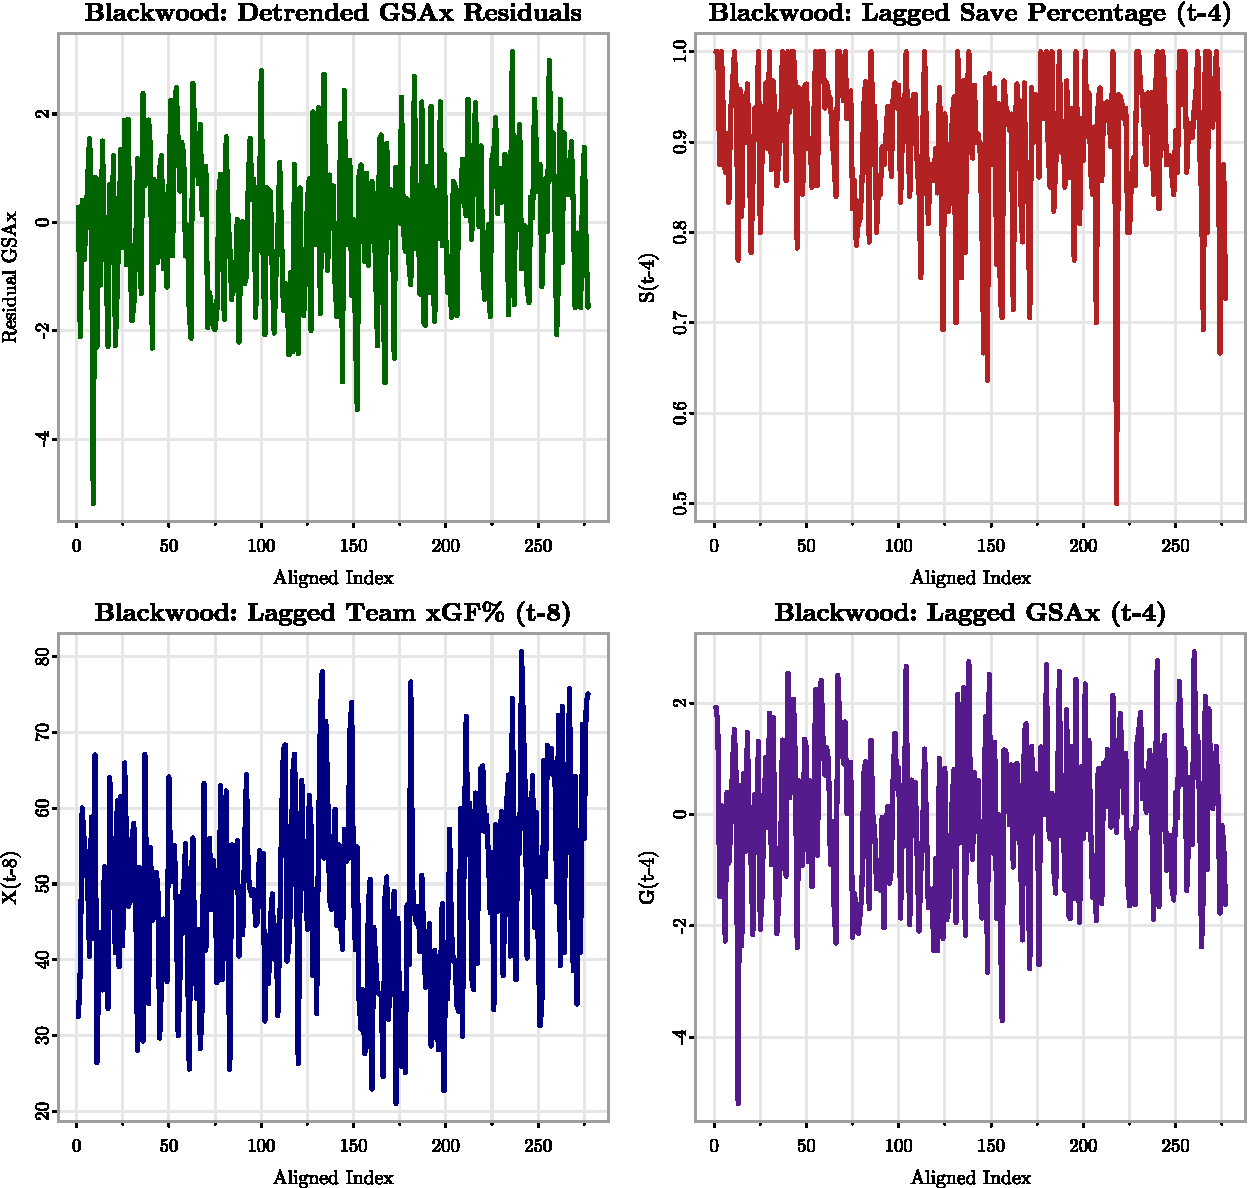
\includegraphics[width=\linewidth]{Homework6_files/figure-latex/pproj-blackwood-plot-1} \end{center}

\begin{center}
\scriptsize
\begin{table}[H]

\caption{\label{tab:pproj-blackwood-diag-table}Blackwood detrended and deseasonalized series diagnostics}
\centering
\begin{tabular}[t]{ccccccc}
\toprule
Series & Mean & Min & Max & 1st-Half Var. & 2nd-Half Var. & 2nd/1st\\
\midrule
$\widehat{\varepsilon}^{(B)}_t$ & 0.0000 & -5.1895 & 3.1494 & 1.9892 & 1.7742 & 0.8919\\
$S_{t-4}$ & 0.9020 & 0.5000 & 1.0000 & 0.0049 & 0.0075 & 1.5534\\
$X_{t-8}$ & 48.4562 & 21.0299 & 80.6570 & 118.8624 & 193.0579 & 1.6242\\
$G_{t-4}$ & -0.0405 & -5.1899 & 2.9214 & 2.0483 & 1.8179 & 0.8875\\
\bottomrule
\end{tabular}
\end{table}
\normalsize
\end{center}

\begin{center}
\small
\begin{table}[H]

\caption{\label{tab:pproj-blackwood-transform-table}Blackwood shifted log and Box-Cox comparison}
\centering
\begin{tabular}[t]{cccccc}
\toprule
Series & Shift & $\hat{\lambda}$ & Raw & Shifted Log & Shifted Box-Cox\\
\midrule
$\widehat{\varepsilon}^{(B)}_t$ & 6.1895 & 1.7045 & 0.8919 & 0.6906 & 0.9521\\
$S_{t-4}$ & 0.0000 & 1.9999 & 1.5534 & 1.8180 & 1.3783\\
$X_{t-8}$ & 0.0000 & 0.8416 & 1.6242 & 1.5845 & 1.6133\\
$G_{t-4}$ & 6.1899 & 1.6718 & 0.8875 & 0.7060 & 0.9339\\
\bottomrule
\end{tabular}
\end{table}
\normalsize
\end{center}

First, the key is that a variance-stabilizing transformation is only needed if the spread still increases with time after detrending and deseasonalizing. The response residual plot does not show marked fanning-out, and its first-half and second-half variances are 1.9892 and 1.7742, giving a variance ratio of 0.8919. So the detrended response already has fairly stable spread. For the aligned predictors, the later-half spread is somewhat larger for \(S_{t-4}\) and \(X_{t-8}\), with variance ratios 1.5534 and 1.6242, but the plots do not show the kind of strong variance growth but rather only some extreme outliers, which is probably driving up this ratio. More importantly, the candidate transformations do not materially improve those ratios. For \(S_{t-4}\), the shifted-log ratio is 1.818 and the shifted Box-Cox ratio is 1.3783, compared with the raw ratio 1.5534. For \(X_{t-8}\), the corresponding values are 1.5845, 1.6133, and 1.6242, which are all very similar. So for Blackwood, the evidence does not support an additional variance-stabilizing transformation. The appropriate final transformation is just mean correction:
\[
\widetilde{\varepsilon}^{(B)}_t = \widehat{\varepsilon}^{(B)}_t - \overline{\widehat{\varepsilon}^{(B)}_t},
\quad
\widetilde{S}_{t-4} = S_{t-4} - \overline{S_{t-4}},
\quad
\widetilde{X}_{t-8} = X_{t-8} - \overline{X_{t-8}},
\quad
\widetilde{G}_{t-4} = G_{t-4} - \overline{G_{t-4}}.
\]
For the response, the mean-only model is
\[
\widehat{\varepsilon}^{(B)}_t = \hat{\mu}_B + W_t,
\qquad
\hat{\mu}_B = 0.000000,
\]
so the centering is essentially zero, as expected. Putting Homework 5 and Homework 6 together, the final fitted Blackwood model remains on the original response scale:
\[
G_t = 0.839751
 -  0.543763 S_{t-4}
 -  0.008309 X_{t-8}
 -  0.082838 G_{t-4}
 + W_t.
\]
Here, \(G_t\) and \(G_{t-4}\) are game-by-game even-strength GSAx in goals, \(S_{t-4}\) is lag-4 game-by-game even-strength save percentage recorded as a proportion, \(X_{t-8}\) is lag-8 team even-strength xGF\% recorded in percentage points, and \(W_t\) is a mean-zero error term.

\begin{Shaded}
\begin{Highlighting}[]
\FunctionTok{with\_family}\NormalTok{(\{}
  \CommentTok{\# Plot Blackwood\textquotesingle{}s final centered response and its ACF to check for leftover mean structure.}
\NormalTok{  op }\OtherTok{\textless{}{-}} \FunctionTok{par}\NormalTok{(}\AttributeTok{no.readonly =} \ConstantTok{TRUE}\NormalTok{)}
  \FunctionTok{on.exit}\NormalTok{(}\FunctionTok{par}\NormalTok{(op), }\AttributeTok{add =} \ConstantTok{TRUE}\NormalTok{)}
  \FunctionTok{par}\NormalTok{(}\AttributeTok{mfrow =} \FunctionTok{c}\NormalTok{(}\DecValTok{1}\NormalTok{, }\DecValTok{2}\NormalTok{), }\AttributeTok{mar =} \FunctionTok{c}\NormalTok{(}\FloatTok{4.2}\NormalTok{, }\FloatTok{4.5}\NormalTok{, }\FloatTok{2.8}\NormalTok{, }\FloatTok{1.2}\NormalTok{), }\AttributeTok{mgp =} \FunctionTok{c}\NormalTok{(}\FloatTok{2.2}\NormalTok{, }\FloatTok{0.7}\NormalTok{, }\DecValTok{0}\NormalTok{), }\AttributeTok{cex.main =} \FloatTok{1.0}\NormalTok{, }\AttributeTok{cex.lab =} \FloatTok{0.95}\NormalTok{, }\AttributeTok{cex.axis =} \FloatTok{0.9}\NormalTok{)}
\NormalTok{  astsa}\SpecialCharTok{::}\FunctionTok{tsplot}\NormalTok{(}\FunctionTok{ts}\NormalTok{(blackwood\_final\_centered, }\AttributeTok{start =} \DecValTok{1}\NormalTok{, }\AttributeTok{frequency =} \DecValTok{1}\NormalTok{), }\AttributeTok{main =} \StringTok{\textquotesingle{}Blackwood: Final Centered Response\textquotesingle{}}\NormalTok{, }\AttributeTok{xlab =} \StringTok{\textquotesingle{}Aligned Index\textquotesingle{}}\NormalTok{, }\AttributeTok{ylab =} \StringTok{\textquotesingle{}Centered Residual\textquotesingle{}}\NormalTok{, }\AttributeTok{col =} \StringTok{\textquotesingle{}darkgreen\textquotesingle{}}\NormalTok{, }\AttributeTok{lwd =} \DecValTok{2}\NormalTok{)}
  \FunctionTok{acf}\NormalTok{(blackwood\_final\_centered, }\AttributeTok{lag.max =} \DecValTok{20}\NormalTok{, }\AttributeTok{main =} \StringTok{\textquotesingle{}\textquotesingle{}}\NormalTok{, }\AttributeTok{col =} \StringTok{\textquotesingle{}darkgreen\textquotesingle{}}\NormalTok{, }\AttributeTok{lwd =} \DecValTok{2}\NormalTok{)}
  \FunctionTok{title}\NormalTok{(}\AttributeTok{main =} \StringTok{\textquotesingle{}Blackwood: Final Response ACF\textquotesingle{}}\NormalTok{)}
\NormalTok{\})}
\end{Highlighting}
\end{Shaded}

\begin{center}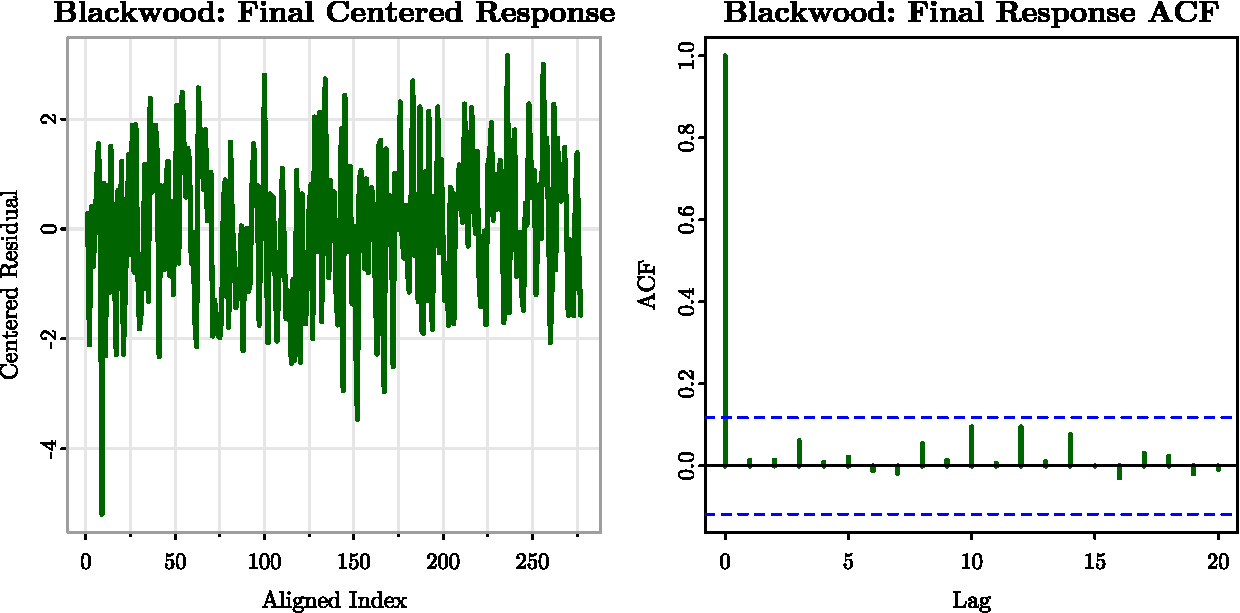
\includegraphics[width=\linewidth]{Homework6_files/figure-latex/pproj-blackwood-final-check-1} \end{center}

After this final mean correction, Blackwood's centered response has sample mean 0.000000. In the time plot, it fluctuates around \(0\) with no obvious remaining pattern in the mean. In the ACF plot, the only clearly dominant value is at lag \(0\), while the remaining autocorrelations stay small overall. Overall, the final series is adequately mean-corrected and random.

\begin{Shaded}
\begin{Highlighting}[]
\FunctionTok{with\_family}\NormalTok{(\{}
  \CommentTok{\# Plot Shesterkin\textquotesingle{}s detrended response and aligned predictors to assess spread over time.}
\NormalTok{  op }\OtherTok{\textless{}{-}} \FunctionTok{par}\NormalTok{(}\AttributeTok{no.readonly =} \ConstantTok{TRUE}\NormalTok{)}
  \FunctionTok{on.exit}\NormalTok{(}\FunctionTok{par}\NormalTok{(op), }\AttributeTok{add =} \ConstantTok{TRUE}\NormalTok{)}
  \FunctionTok{par}\NormalTok{(}\AttributeTok{mfrow =} \FunctionTok{c}\NormalTok{(}\DecValTok{2}\NormalTok{, }\DecValTok{2}\NormalTok{), }\AttributeTok{mar =} \FunctionTok{c}\NormalTok{(}\FloatTok{4.2}\NormalTok{, }\FloatTok{4.5}\NormalTok{, }\FloatTok{2.8}\NormalTok{, }\FloatTok{1.2}\NormalTok{), }\AttributeTok{mgp =} \FunctionTok{c}\NormalTok{(}\FloatTok{2.2}\NormalTok{, }\FloatTok{0.7}\NormalTok{, }\DecValTok{0}\NormalTok{), }\AttributeTok{cex.main =} \FloatTok{1.0}\NormalTok{, }\AttributeTok{cex.lab =} \FloatTok{0.95}\NormalTok{, }\AttributeTok{cex.axis =} \FloatTok{0.9}\NormalTok{)}
\NormalTok{  astsa}\SpecialCharTok{::}\FunctionTok{tsplot}\NormalTok{(}\FunctionTok{ts}\NormalTok{(shesterkin\_resid, }\AttributeTok{start =} \DecValTok{1}\NormalTok{, }\AttributeTok{frequency =} \DecValTok{1}\NormalTok{), }\AttributeTok{main =} \StringTok{\textquotesingle{}Shesterkin: Detrended GSAx Residuals\textquotesingle{}}\NormalTok{, }\AttributeTok{xlab =} \StringTok{\textquotesingle{}Aligned Index\textquotesingle{}}\NormalTok{, }\AttributeTok{ylab =} \StringTok{\textquotesingle{}Residual GSAx\textquotesingle{}}\NormalTok{, }\AttributeTok{col =} \StringTok{\textquotesingle{}darkgreen\textquotesingle{}}\NormalTok{, }\AttributeTok{lwd =} \DecValTok{2}\NormalTok{)}
\NormalTok{  astsa}\SpecialCharTok{::}\FunctionTok{tsplot}\NormalTok{(}\FunctionTok{ts}\NormalTok{(shesterkin\_hw5}\SpecialCharTok{$}\NormalTok{data}\SpecialCharTok{$}\NormalTok{sv, }\AttributeTok{start =} \DecValTok{1}\NormalTok{, }\AttributeTok{frequency =} \DecValTok{1}\NormalTok{), }\AttributeTok{main =} \StringTok{\textquotesingle{}Shesterkin: Lagged Save Percentage (t{-}2)\textquotesingle{}}\NormalTok{, }\AttributeTok{xlab =} \StringTok{\textquotesingle{}Aligned Index\textquotesingle{}}\NormalTok{, }\AttributeTok{ylab =} \StringTok{\textquotesingle{}S(t{-}2)\textquotesingle{}}\NormalTok{, }\AttributeTok{col =} \StringTok{\textquotesingle{}firebrick\textquotesingle{}}\NormalTok{, }\AttributeTok{lwd =} \DecValTok{2}\NormalTok{)}
\NormalTok{  astsa}\SpecialCharTok{::}\FunctionTok{tsplot}\NormalTok{(}\FunctionTok{ts}\NormalTok{(shesterkin\_hw5}\SpecialCharTok{$}\NormalTok{data}\SpecialCharTok{$}\NormalTok{xgf, }\AttributeTok{start =} \DecValTok{1}\NormalTok{, }\AttributeTok{frequency =} \DecValTok{1}\NormalTok{), }\AttributeTok{main =} \StringTok{\textquotesingle{}Shesterkin: Lagged Team xGF\% (t{-}4)\textquotesingle{}}\NormalTok{, }\AttributeTok{xlab =} \StringTok{\textquotesingle{}Aligned Index\textquotesingle{}}\NormalTok{, }\AttributeTok{ylab =} \StringTok{\textquotesingle{}X(t{-}4)\textquotesingle{}}\NormalTok{, }\AttributeTok{col =} \StringTok{\textquotesingle{}navy\textquotesingle{}}\NormalTok{, }\AttributeTok{lwd =} \DecValTok{2}\NormalTok{)}
\NormalTok{  astsa}\SpecialCharTok{::}\FunctionTok{tsplot}\NormalTok{(}\FunctionTok{ts}\NormalTok{(shesterkin\_hw5}\SpecialCharTok{$}\NormalTok{data}\SpecialCharTok{$}\NormalTok{gLag, }\AttributeTok{start =} \DecValTok{1}\NormalTok{, }\AttributeTok{frequency =} \DecValTok{1}\NormalTok{), }\AttributeTok{main =} \StringTok{\textquotesingle{}Shesterkin: Lagged GSAx (t{-}2)\textquotesingle{}}\NormalTok{, }\AttributeTok{xlab =} \StringTok{\textquotesingle{}Aligned Index\textquotesingle{}}\NormalTok{, }\AttributeTok{ylab =} \StringTok{\textquotesingle{}G(t{-}2)\textquotesingle{}}\NormalTok{, }\AttributeTok{col =} \StringTok{\textquotesingle{}purple4\textquotesingle{}}\NormalTok{, }\AttributeTok{lwd =} \DecValTok{2}\NormalTok{)}
\NormalTok{\})}
\end{Highlighting}
\end{Shaded}

\begin{center}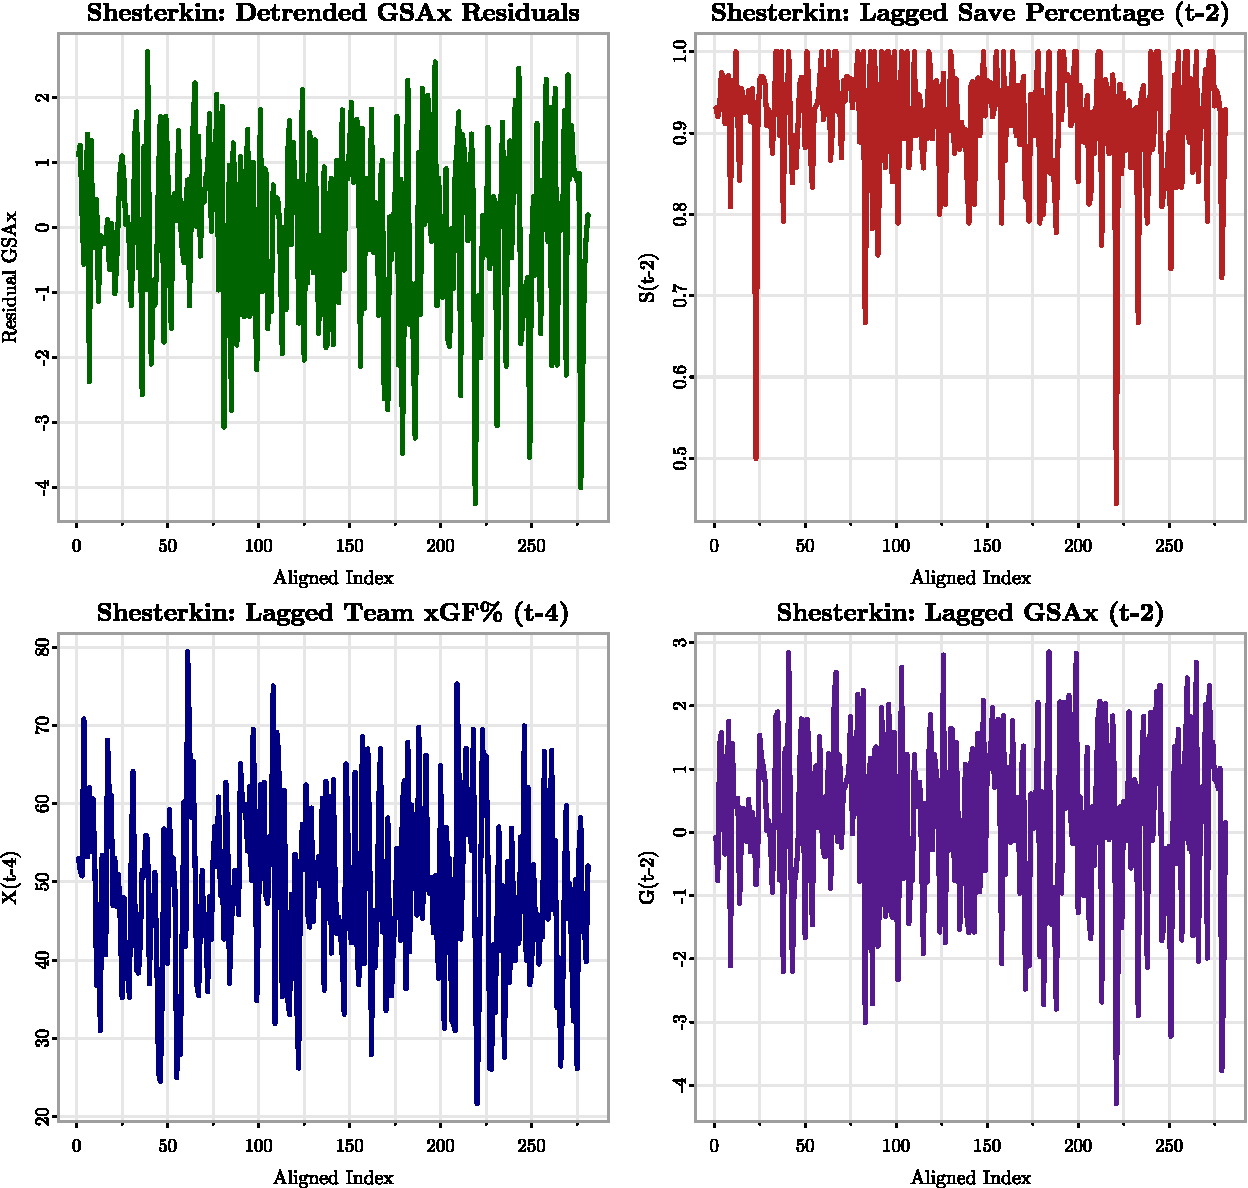
\includegraphics[width=\linewidth]{Homework6_files/figure-latex/pproj-shesterkin-plot-1} \end{center}

\begin{center}
\scriptsize
\begin{table}[H]

\caption{\label{tab:pproj-shesterkin-diag-table}Shesterkin detrended and deseasonalized series diagnostics}
\centering
\begin{tabular}[t]{ccccccc}
\toprule
Series & Mean & Min & Max & 1st-Half Var. & 2nd-Half Var. & 2nd/1st\\
\midrule
$\widehat{\varepsilon}^{(S)}_t$ & 0.0000 & -4.2455 & 2.7080 & 1.3668 & 2.1710 & 1.5884\\
$S_{t-2}$ & 0.9161 & 0.4444 & 1.0000 & 0.0048 & 0.0062 & 1.2784\\
$X_{t-4}$ & 49.0086 & 21.6791 & 79.4161 & 116.5492 & 131.4910 & 1.1282\\
$G_{t-2}$ & 0.2355 & -4.2880 & 2.8570 & 1.4791 & 2.2075 & 1.4924\\
\bottomrule
\end{tabular}
\end{table}
\normalsize
\end{center}

\begin{center}
\small
\begin{table}[H]

\caption{\label{tab:pproj-shesterkin-transform-table}Shesterkin shifted log and Box-Cox comparison}
\centering
\begin{tabular}[t]{cccccc}
\toprule
Series & Shift & $\hat{\lambda}$ & Raw & Shifted Log & Shifted Box-Cox\\
\midrule
$\widehat{\varepsilon}^{(S)}_t$ & 5.2455 & 1.9999 & 1.5884 & 2.1539 & 1.4136\\
$S_{t-2}$ & 0.0000 & 1.9999 & 1.2784 & 1.3387 & 1.2456\\
$X_{t-4}$ & 0.0000 & 0.3105 & 1.1282 & 1.1515 & 1.1432\\
$G_{t-2}$ & 5.2880 & 1.9999 & 1.4924 & 1.9579 & 1.3344\\
\bottomrule
\end{tabular}
\end{table}
\normalsize
\end{center}

For Shesterkin, the plot evidence is a little different. In the detrended response residuals \(\widehat{\varepsilon}^{(S)}_t\), and also in the lagged response predictor \(G_{t-2}\), the later part of the series does show mild fanning-out. This is consistent with the variance ratios: for \(\widehat{\varepsilon}^{(S)}_t\), the first-half and second-half variances are 1.3668 and 2.171, giving ratio 1.5884; for \(G_{t-2}\), the ratio is 1.4924. So for Shesterkin, some additional variance stabilization is reasonable for those two series. Among the candidate transformations, the shifted log does not help, since it raises the variance ratios to 2.1539 for \(\widehat{\varepsilon}^{(S)}_t\) and 1.9579 for \(G_{t-2}\). The shifted Box-Cox transformation improves them to 1.4136 and 1.3344, respectively, which is better than the raw scale in both cases. Therefore, for Shesterkin I use an additional shifted Box-Cox transformation for the detrended response residuals and for \(G_{t-2}\):
\[
Y^{(S,\varepsilon)}_t
= \frac{\left(\widehat{\varepsilon}^{(S)}_t + c_{\varepsilon}\right)^{\lambda_{\varepsilon}} - 1}{\lambda_{\varepsilon}},
\qquad
c_{\varepsilon} = 5.2455,
\qquad
\lambda_{\varepsilon} = 1.9999,
\]
and
\[
Y^{(S,G)}_t
= \frac{\left(G_{t-2} + c_G\right)^{\lambda_G} - 1}{\lambda_G},
\qquad
c_G = 5.288,
\qquad
\lambda_G = 1.9999.
\]

For \(S_{t-2}\) and \(X_{t-4}\), I do not transform. Their variance ratios are only 1.2784 and 1.1282, and the candidate transformed versions do not improve them enough to justify changing scale. So for Shesterkin, the final transformed set is
\[
Y^{(S,\varepsilon)}_t,\quad S_{t-2},\quad X_{t-4},\quad Y^{(S,G)}_t.
\]
At the end, just like Blackwood, I also do the mean correction. So the final centered set is
\[
\widetilde{Y}^{(S,\varepsilon)}_t = Y^{(S,\varepsilon)}_t - \overline{Y^{(S,\varepsilon)}_t},
\quad
\widetilde{S}_{t-2} = S_{t-2} - \overline{S_{t-2}},
\quad
\widetilde{X}_{t-4} = X_{t-4} - \overline{X_{t-4}},
\quad
\widetilde{Y}^{(S,G)}_t = Y^{(S,G)}_t - \overline{Y^{(S,G)}_t}.
\]
For the transformed response series, the mean-only correction is
\[
Y^{(S,\varepsilon)}_t = \mu_{S,\varepsilon} + W_t,
\qquad
\mu_{S,\varepsilon} = 14.136084,
\]
and for the transformed lagged GSAx series,
\[
\overline{Y^{(S,G)}_t} = 15.669290.
\]

Putting Homework 5 and Homework 6 together, the final fitted Shesterkin model is written in two parts. The fitted lagged-regression mean equation from Homework 5 is
\[
G_t = 1.968206
 -  2.333501 S_{t-2}
 +  0.008648 X_{t-4}
 -  0.054451 G_{t-2}
 + \widehat{\varepsilon}^{(S)}_t,
\]
where \(G_t\) and \(G_{t-2}\) are game-by-game even-strength GSAx in goals, \(S_{t-2}\) is lag-2 game-by-game even-strength save percentage recorded as a proportion, and \(X_{t-4}\) is lag-4 team even-strength xGF\% recorded in percentage points. Homework 6 then treats the remaining response-side error by
\[
Y^{(S,\varepsilon)}_t
= \frac{\left(\widehat{\varepsilon}^{(S)}_t + 5.2455\right)^{1.9999} - 1}{1.9999}
= 14.136084 + W_t,
\]
with \(W_t\) denoting the final mean-zero white-noise term after the transformation and mean correction.

\begin{Shaded}
\begin{Highlighting}[]
\FunctionTok{with\_family}\NormalTok{(\{}
  \CommentTok{\# Plot Shesterkin\textquotesingle{}s final centered transformed response and its ACF to check for leftover mean structure.}
\NormalTok{  op }\OtherTok{\textless{}{-}} \FunctionTok{par}\NormalTok{(}\AttributeTok{no.readonly =} \ConstantTok{TRUE}\NormalTok{)}
  \FunctionTok{on.exit}\NormalTok{(}\FunctionTok{par}\NormalTok{(op), }\AttributeTok{add =} \ConstantTok{TRUE}\NormalTok{)}
  \FunctionTok{par}\NormalTok{(}\AttributeTok{mfrow =} \FunctionTok{c}\NormalTok{(}\DecValTok{1}\NormalTok{, }\DecValTok{2}\NormalTok{), }\AttributeTok{mar =} \FunctionTok{c}\NormalTok{(}\FloatTok{4.2}\NormalTok{, }\FloatTok{4.5}\NormalTok{, }\FloatTok{2.8}\NormalTok{, }\FloatTok{1.2}\NormalTok{), }\AttributeTok{mgp =} \FunctionTok{c}\NormalTok{(}\FloatTok{2.2}\NormalTok{, }\FloatTok{0.7}\NormalTok{, }\DecValTok{0}\NormalTok{), }\AttributeTok{cex.main =} \FloatTok{1.0}\NormalTok{, }\AttributeTok{cex.lab =} \FloatTok{0.95}\NormalTok{, }\AttributeTok{cex.axis =} \FloatTok{0.9}\NormalTok{)}
\NormalTok{  astsa}\SpecialCharTok{::}\FunctionTok{tsplot}\NormalTok{(}\FunctionTok{ts}\NormalTok{(shesterkin\_final\_centered, }\AttributeTok{start =} \DecValTok{1}\NormalTok{, }\AttributeTok{frequency =} \DecValTok{1}\NormalTok{), }\AttributeTok{main =} \StringTok{\textquotesingle{}Shesterkin: Final Centered Response\textquotesingle{}}\NormalTok{, }\AttributeTok{xlab =} \StringTok{\textquotesingle{}Aligned Index\textquotesingle{}}\NormalTok{, }\AttributeTok{ylab =} \StringTok{\textquotesingle{}Centered Transformed Response\textquotesingle{}}\NormalTok{, }\AttributeTok{col =} \StringTok{\textquotesingle{}darkgreen\textquotesingle{}}\NormalTok{, }\AttributeTok{lwd =} \DecValTok{2}\NormalTok{)}
  \FunctionTok{acf}\NormalTok{(shesterkin\_final\_centered, }\AttributeTok{lag.max =} \DecValTok{20}\NormalTok{, }\AttributeTok{main =} \StringTok{\textquotesingle{}\textquotesingle{}}\NormalTok{, }\AttributeTok{col =} \StringTok{\textquotesingle{}darkgreen\textquotesingle{}}\NormalTok{, }\AttributeTok{lwd =} \DecValTok{2}\NormalTok{)}
  \FunctionTok{title}\NormalTok{(}\AttributeTok{main =} \StringTok{\textquotesingle{}Shesterkin: Final Response ACF\textquotesingle{}}\NormalTok{)}
\NormalTok{\})}
\end{Highlighting}
\end{Shaded}

\begin{center}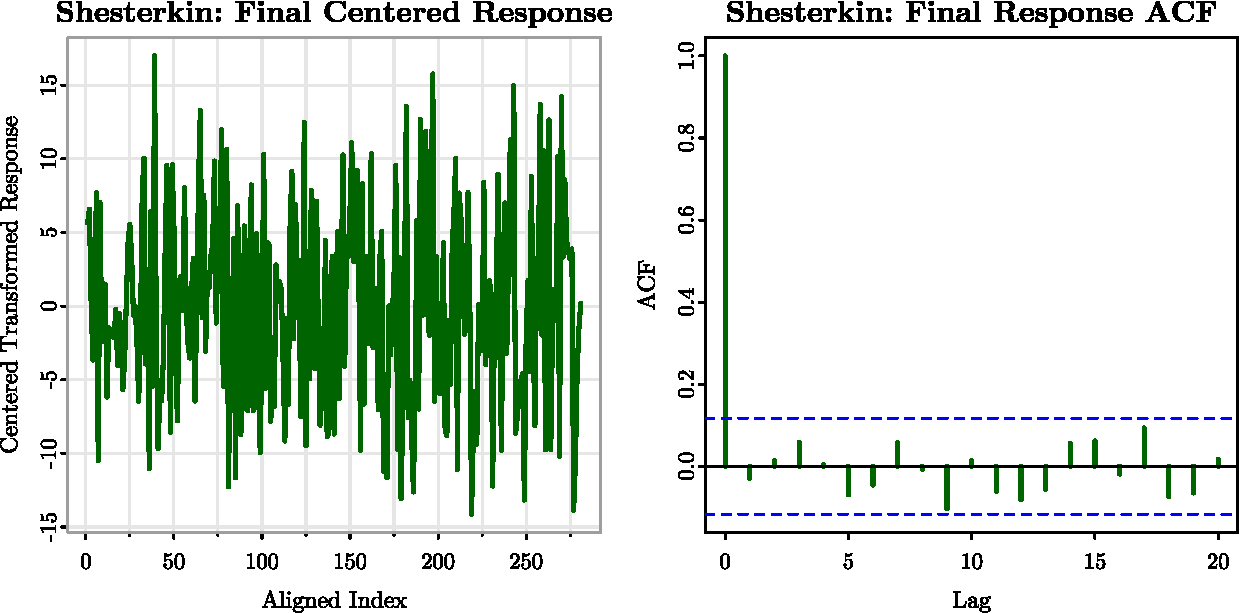
\includegraphics[width=\linewidth]{Homework6_files/figure-latex/pproj-shesterkin-final-check-1} \end{center}

After the shifted Box-Cox step and the final mean correction, Shesterkin's centered response has sample mean 0.000000. In the time plot, it fluctuates around \(0\) with no obvious remaining pattern in the mean. In the ACF plot, the only clearly dominant value is at lag \(0\), while the remaining autocorrelations stay small overall. So for Shesterkin, the final transformed response series is also adequately mean-corrected and random.

\end{document}
